\documentclass[main.tex]{subfiles}
\begin{document}


\chapter{Double beta decay}
 

%\begin{flushright}
%\textit{Nothing contributes so much to tranquillize the mind \\
%as a steady purpose, a point on which the soul \\
%can focus its intellectual eye.}\\
%Mary Shelley, \textit{Frankenstein}.
%\end{flushright} 


\NI Since the prediction of the neutrino in 1930 and their first detection in 1956, many studies have been done to understand their properties. One of the most important achievements is the discovery of their oscillations, proving their non-zero mass which is a first indication of physics beyond Standard Model. There are still remaining questions in neutrino physics including their nature and how they acquire their masses. Since it has been proven that the neutrinoless double beta decay necessarily involves Majorana neutrino, the search for this hypothetical decay is one of the most active research topics in neutrino physics. Its observation may also give access to their absolute mass scale.


\bigskip


\NI Some elements on simple beta decay and double beta decay are respectively introduced in Sections~\ref{sec:betaDecay} and~\ref{sec:2NeutrinoDBD}. The neutrinoless double beta decay is discussed in Section~\ref{sec:0NeutrinoDBD}. The different double beta decay experiments and the status of the searches are respectively presented in Section~\ref{sec:DBDexperiment} and~\ref{sec:StatusDBD}.


\section{Beta decay}\label{sec:betaDecay}


\NI Beta decay is a radioactive decay which transmutes a nucleus into a different one. This decay is mediated by the weak interaction and is always accompanied by a neutrino or antineutrino emission. Beta decays have been sorted in three categories~:


\bigskip


\NI $\boldsymbol{\beta^-}$ \textbf{decay}, in which a neutron converts into a proton with the emission of an electron and an antineutrino~:
\begin{equation}
\text{n} \rightarrow \text{p} + \text{e}^- + \bar{\nu}_\text{e}
\end{equation}


\bigskip


\NI $\boldsymbol{\beta^+}$ \textbf{decay}, in which a proton converts into a neutron with the emission of an positron and a neutrino~:
\begin{equation}
\text{p} \rightarrow \text{n} + \text{e}^+ + \nu_\text{e}
\end{equation}  


\bigskip
 
 
\NI \textbf{Electron capture (EC)}, in which an atomic electron is captured by its nucleus, resulting in the emission of a single neutrino~:
\begin{equation}
\text{p} + \text{e}^- \rightarrow \text{n} + \nu_{\text{e}}
\end{equation} 


\bigskip


\NI Note that there is a competition between the $\beta^+$ decay and the electron capture processes. In case the $\beta^+$ decay is forbidden or highly suppressed, the electron capture is the only way for a nuclei to become more stable. After an electron capture, a hole appears in the atomic orbital and the reorganisation of the remaining electrons is accompanied by a cascade of photons and/or Auger electrons. From a kinematic point of view, the released energy in $\beta^{\pm}$ decays is shared between the $\beta$-particle and the neutrino or the antineutrino while, in electron captures, the emitted neutrino carries away all the released energy. The $\beta^{\pm}$ decays can only occur if the mass of the daughter nucleus, $\mathcal{M}$(A,Z$_\text{f}$), is lower than the mother nucleus, $\mathcal{M}$(A,Z$_\text{i}$), where A is the number of nucleons and Z is the atomic number. The mass of an atomic nucleus is given by : 


\begin{equation}\label{eq:Mass}
\mathcal{M} (\text{A},\text{Z}) = \text{Z} \text{m}_\text{p} + (\text{A}-\text{Z}) \text{m}_\text{n} - \text{E}_\text{B}
\end{equation}


\bigskip


\NI where m$_\text{p}$ is the mass of the proton, m$_\text{n}$ is the mass of the neutron and E$_\text{B}$ is the binding energy of the nucleus which can be estimated with the semi-empirical mass formula also called Bethe–Weizsäcker formula~\cite{WeizsckerFormula} :  


\begin{equation}\label{eq:EB}
\text{E}_\text{B} = \text{a}_\text{v} \text{A} - \text{a}_\text{s} \text{A}^{\text{2/3}} -  \text{a}_\text{c} \frac{\text{Z}^\text{2}}{\text{A}^{\text{1/3}}} - \text{a}_\text{A} \frac{(\text{A}-\text{2Z})^\text{2}}{\text{A}} + \delta \text{(A,Z)} 
\end{equation}


\bigskip


\NI where a$_\text{v}$A is known as the volume term. It represents the interaction of a nucleon with its nearest neighbors via the strong nuclear force. It is proportional to A and does not depend on Z. The surface term, a$_\text{s}$A$^{\text{2/3}}$, also based on the strong interaction, is a correction to the volume term. It takes into account the fact that the nucleons on the surface of the nucleus have less nearest neighbors to interact with compared to the nucleons located inside the nucleus. The third term, (a$_\text{c}$ Z$^\text{2}$)/A$^{\text{1/3}}$, known as the Coulomb term, takes into account the electrostatic repulsion between protons. The fourth term, a$_\text{A}$(A-2Z)$^\text{2}$/A is the asymmetry term. Based on the Pauli exclusion principle, this term has been added to take into account the asymmetry between the number of protons and neutrons in the nucleus. This term is equal to zero when a nucleus has the same number of protons and neutrons. The last term $\delta$ which is called pairing term, takes into account the effect of spin-coupling. Indeed, due to the Pauli exclusion principle, the energy of a nucleus is minimised in the case the number of protons with spin up is equal to the number of protons with spin down. As it is similar for the neutron the pairing term is written : 


\begin{equation}
\delta \text{(A,Z)} = 
\left\{
\begin{array}{l}
  +\delta_0~\text{if~A is even}~:~\text{Z}~\text{and}~(\text{A}-\text{Z})~\text{even} \\[0.3cm]
  \text{0}~\text{if~A~is odd}\\[0.3cm]
  -\delta_0~\text{if~A is even}~:~\text{Z}~\text{and}~(\text{A}-\text{Z})~\text{odd}
\end{array}
\right.
\end{equation}


\bigskip


\NI Finally, by combining Eq~\ref{eq:Mass} and Eq~\ref{eq:EB}, the mass of an atomic nucleus can be written~as~:


\begin{equation}\label{eq:MassFinal}
\mathcal{M} (\text{A},\text{Z}) = \text{Z}\text{m}_\text{p} + \text{(A - Z)}\text{m}_{\text{n}} - \text{a}_\text{v} \text{A} + \text{a}_\text{s} \text{A}^{\text{2/3}} +  \text{a}_\text{c} \frac{\text{Z}^\text{2}}{\text{A}^{\text{1/3}}} +  \text{a}_\text{A} \frac{\text{(A-2Z)}^\text{2}}{\text{A}} + \delta \text{(A,Z)} 
\end{equation}


\NI It can be deduced from~\ref{eq:MassFinal} that at a given A, parabolic curves are generated as a function of Z and provide which $\beta$ decays are energetically allowed or forbidden. In case A is odd, only one curve exists, but for an even A, two curves exist split by the pairing term as shown in Figure~\ref{WeizsackerParabola}. It can also be seen that the $\beta^-$ decays $^{\text{82}}$Ge $\rightarrow$ $^{\text{82}}$As and $^{\text{82}}$As $\rightarrow$ $^{\text{82}}$Se are energetically allowed while the $\beta^-$ decay $^{\text{82}}$Se~$\rightarrow$~$^{\text{82}}$Br is forbidden.


\begin{figure}[h!]
\begin{center}
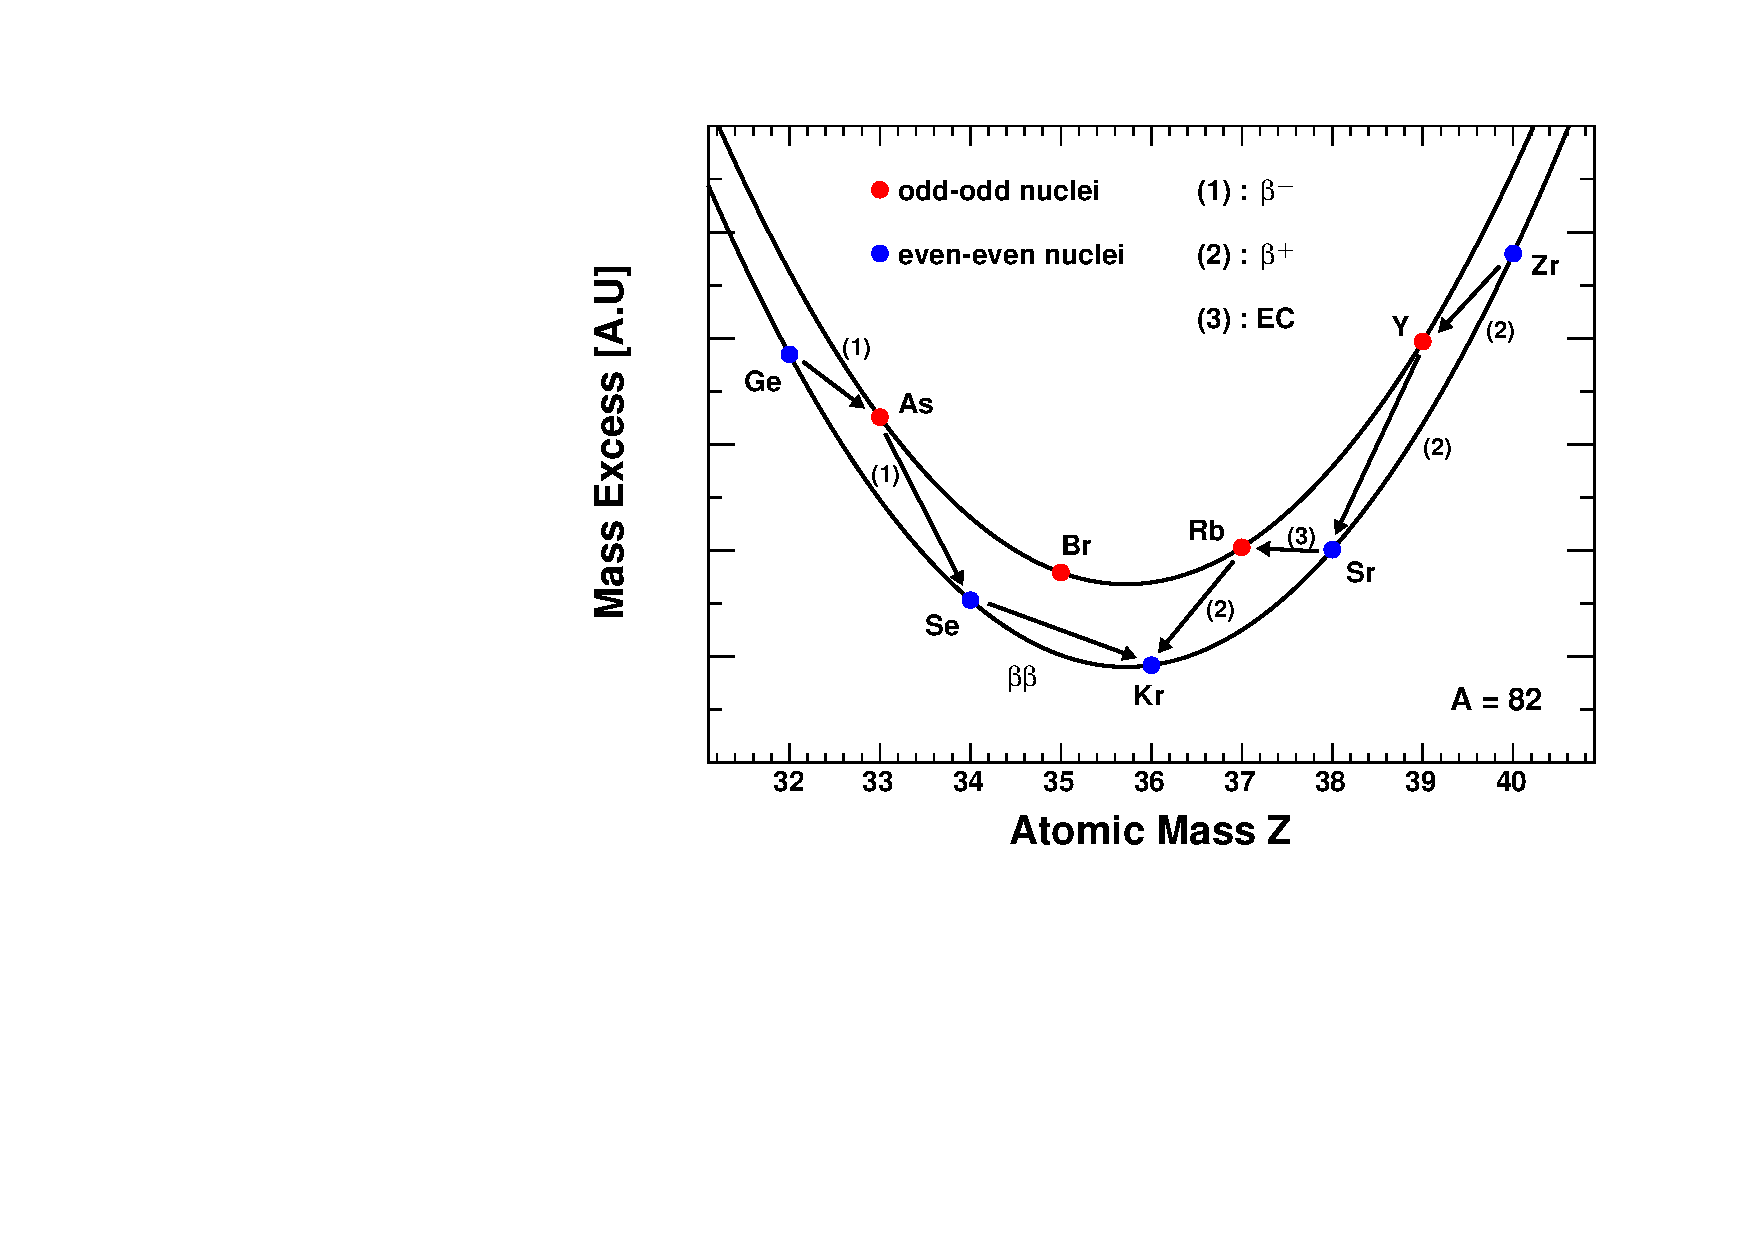
\includegraphics[scale=0.55]{pictures/Chap2/WeizsackerParabola_v4.pdf}
\caption{Mass excess according to the atomic number Z estimated with the Bethe–Weizsäcker formula at A = 82. 2$\nu\beta\beta$~decay of $^{\text{82}}$Se is possible because its simple $\beta$ decay is energetically forbidden.}
\label{WeizsackerParabola}
\end{center}
\end{figure}


\FloatBarrier



\section{Two Neutrino Double Beta Decay}\label{sec:2NeutrinoDBD}


\NI As shown in Figure~\ref{WeizsackerParabola}, $^{\text{82}}$Se is stable against $\beta$ decay but has the possibility to undergo two neutrino double beta decay (2$\nu\beta\beta$) to reach a more stable state. This decay, proposed by Goeppert-Mayer in 1935~\cite{GoeppertMayerDoubleBetaDecay}, is a rare process in which 2$\beta^{-}$ or 2$\beta^{+}$ decays happen simulataneously~: 


\begin{equation}
\begin{split}
\mathcal{N} (\text{A,Z}) \rightarrow \mathcal{N} (\text{A,Z+2}) + \text{2e}^- + \text{2}\bar{\nu}_{\text{e}}  \\[0.1cm]
\mathcal{N} (\text{A,Z}) \rightarrow \mathcal{N} (\text{A,Z}-\text{2}) + \text{2e}^+ + \text{2}\nu_{\text{e}} 
\end{split}
\end{equation}


\NI The 2$\nu\beta\beta$~decay is a second order process allowed in SM and possible only for the even-even nucleus, as it can be seen in Figure~\ref{WeizsackerParabola}. The double $\beta^{+}$ decays are also possible in theory but rarely studied since there are in competition with the double electron capture which makes their half-lives longer than double $\beta^{-}$ decays. The Feynman diagram of 2$\nu\beta\beta$ decay is shown in Figure~\ref{2nubbFeynman}. As the antineutrinos carry away a part of the energy, the total energy of the emitted electrons is a continuous spectrum with an end-point at the nuclear transition energy, Q$_{\beta\beta}$, defined as :


\begin{equation}
\text{Q}_{\beta\beta} = \mathcal{M}_\text{i} - (\mathcal{M}_\text{f} + \text{2m}_\text{e})
\end{equation}


\begin{figure}[h!]
\begin{center}
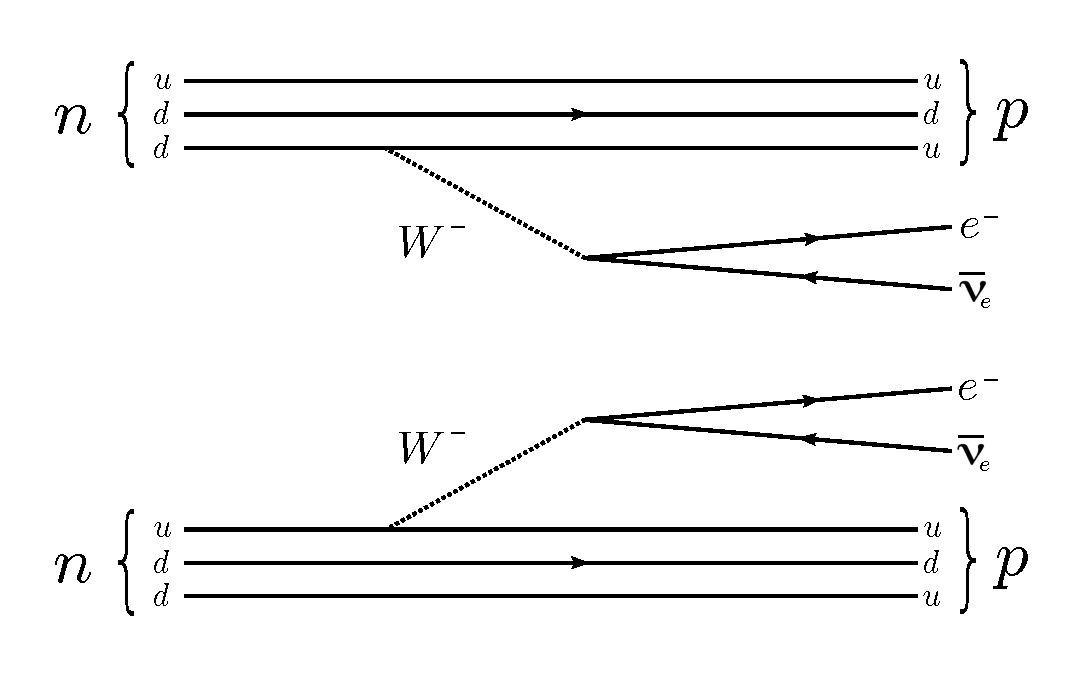
\includegraphics[scale=0.45]{pictures/Chap2/2nubbFeynmanDiagram_v3.pdf}
\caption{Feynman diagram for 2$\nu\beta\beta$ decay. In this second order process, 2 neutrons decay simultaneously (2n $\rightarrow$ 2p + 2e$^-$ + 2$\bar{\nu}$). Two electrons and two anti-neutrinos are emitted.}
\label{2nubbFeynman}
\end{center}
\end{figure}


\NI where $\mathcal{M}_\text{i}$ is the mass of the mother nucleus, $\mathcal{M}_\text{f}$ the mass of the daughter nucleus and m$_\text{e}$ is the electron mass. The shape of this spectrum is shown in Figure~\ref{EnergySpectrumDBD}. The half-life of 2$\nu\beta\beta$ is very long, it depends on the isotope but the orders of magnitude are in the range [10$^{\text{18}}$ - 10$^{\text{24}}$]~y.  The half-life of the decay can be parametrised as : 


\begin{equation}\label{eq:decayRate2nu}
(\text{T}_{\text{1/2}}^{\text{2}\nu})^{\text{-1}} = \text{G}_{\text{2}\nu}(\text{Q}_{\beta\beta}, \text{Z}) \times |\text{M}_{\text{2}\nu}|^\text{2}
\end{equation}


\bigskip


\NI where G$_{\text{2}\nu}$ is the four-body phase space factor that can be calculated analytically and M$_{\text{2}\nu}$ is the nuclear matrix element (NME) for the decay. More details about NME will be given in Section~\ref{sec:NME}.


\bigskip


\NI 41 natural isotopes capable of 2$\nu\beta\beta$~decay exist, 35 by double $\beta^{-}$ and 6 by $\beta^{+}$. The decay rate of 12 of them have been experimentally observed. The transition energy, the natural abundance and the space phase factors of the 35 $\beta^{-}$ isotopes are gathered in~Table~\ref{tab:2nuIsotopes} at the end of the chapter.



\FloatBarrier


\section{Neutrinoless Double Beta Decay}\label{sec:0NeutrinoDBD}


\NI The neutrinoless double beta decay (0$\nu\beta\beta$) is a hypothetical process, in which 2$\beta^{-}$ decays occur simultaneously and no neutrino are emitted :


\begin{equation}
\mathcal{N} (\text{A,Z}) \rightarrow \mathcal{N} (\text{A,Z+2}) + \text{2e}^- 
\end{equation}


\bigskip


\NI Violating lepton number conservation this decay is forbidden in SM and has never been observed. As this decay is only possible if neutrinos are massive and are Majorana particles, it constitutes a sensitive method for testing the Majorana nature of neutrinos~\cite{RacahNeutrinolessDBDMajorana}. All candidates for 2$\nu\beta\beta$~decay are also candidates for 0$\nu\beta\beta$~decay and, a priori, there is no correlation between the two decay rates. 


\bigskip



\NI Many hypothetical mechanisms might mediate the 0$\nu\beta\beta$~decay. The most common of them are the neutrino mass mechanism, right-handed current and Majoron emission modes presented in Sections~\ref{sec:NMM} and~\ref{sec:OtherMechanisms}. In these mechanisms it is clear that the neutrino must be a Majorana particle. But other mechanisms exist, not presented herein, such as R-parity violating supersymmetry~\cite{SUSYandDBD}. In some of these mechanisms, no neutrinos are involved and it is not evident that 0$\nu\beta\beta$~decay confirms the Majorana nature of neutrino~\cite{SUSYandDBD}. In 1980, Schechter and Valle introduced a "black box" diagram depicting this decay~\cite{SchechterValle}. This black box is shown in~Figure~\ref{0nubbBlackBox} and demonstrates that regardless of the underlying mechanism, the 0$\nu\beta\beta$ decay requires Majorana neutrinos.  


\smallskip

\begin{figure}[h!]
\begin{center}
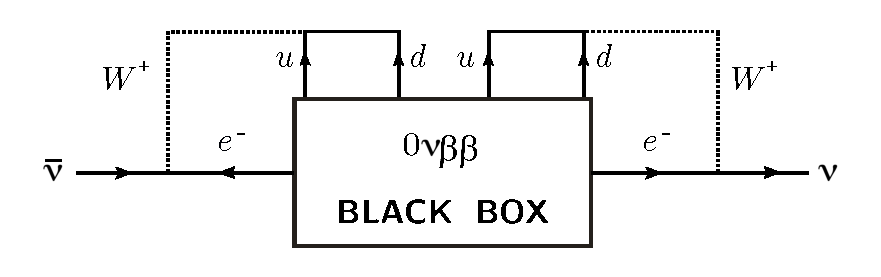
\includegraphics[scale=0.75]{pictures/Chap2/0nubbBlackBox.pdf}
\caption{Black box representing the fact that whatever the underlying mechanism, the observation of the 0$\nu\beta\beta$~decay implies Majorana neutrino.}
\label{0nubbBlackBox}
\end{center}
\end{figure}


\bigskip


\NI As in 2$\nu\beta\beta$, the half-life of 0$\nu\beta\beta$ can be parametrised as : 


\begin{equation}\label{eq:halflife0nu}
(\text{T}_{\text{1/2}}^{\text{0}\nu})^{\text{-1}} = \text{G}_{\text{0}\nu}\text{(Q}_{\beta\beta},\text{Z)} \times \text{M}^\text{2}_{\text{0}\nu} \times \eta^\text{2}
\end{equation}


\bigskip


\NI where G$_{\text{0}\nu}$ is a two-body phase space factor which is well kwown, M$^\text{2}_{\text{0}\nu}$ is the 0$\nu\beta\beta$ NME, and $\eta$ is a lepton violating number parameter which takes into account all the physics behind the 0$\nu\beta\beta$ mechanism. This parameter varies according to the mechanism via which 0$\nu\beta\beta$ is mediated.  


\FloatBarrier


\subsection{Neutrino Mass Mechanism}\label{sec:NMM}



\NI The most common decay model which deviates the least from the SM is the neutrino mass mechanism. In this mechanism, 0$\nu\beta\beta$ is mediated by the exchange of a light neutrino. A Feynman diagram using only SM vertices can be drawn, as shown in Figure~\ref{0nubbNMM}. A right helicity Majorana neutrino is emitted from a W boson and absorbed by another as a left helicity Majorana neutrino. 


\begin{figure}[h!]
\begin{center}
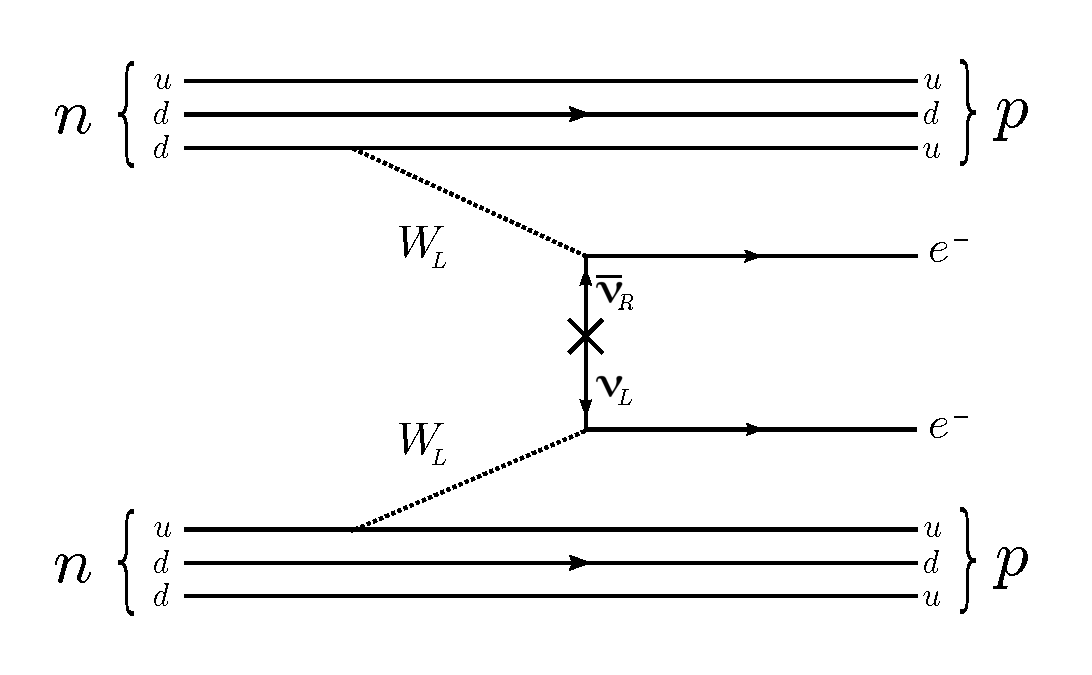
\includegraphics[scale=0.45]{pictures/Chap2/0nubbFeynmanDiagram_NMM.pdf}
\caption{Feynman diagram of 0$\nu\beta\beta$ decay in case of light Majorana neutrino exchange. The emitted electrons carry over all the energy, the experimental signature is given by a peaked distribution at the Q$_{\beta\beta}$ value.}
\label{0nubbNMM}
\end{center}
\end{figure}


\NI In this model, the $\eta$ parameter is given by the effective neutrino mass (m$_{\beta\beta}$) and the half-life can be expressed as: 


\begin{equation}\label{eq:HalfLife0nuParam}
(\text{T}_{\text{1/2}}^{\text{0}\nu})^{\text{-1}} = \text{G}_{\text{0}\nu}\text{(Q}_{\beta\beta},\text{Z)} \times \text{M}^\text{2}_{\text{0}\nu} \times \left( \frac{\text{m}_{\beta\beta}}{\text{m}_\text{e}} \right)^\text{2}
\end{equation}


\bigskip


\NI where m$_\text{e}$ is the electron mass, and m$_{\beta\beta}$ can be written as a function of PMNS matrix elements and neutrino masses (m$_{\nu_\text{\i}}$) : 


\begin{equation}
\begin{split}
\text{m}_{\beta\beta} & = |\sum_\text{i}U_{\text{ei}}^\text{2}~\text{m}_{\nu_\text{i}} | \\
 & = \text{cos}^\text{2}\theta_{\text{12}}~\text{cos}^\text{2}\theta_{\text{13}}~\text{m}_\text{1} + \text{sin}^\text{2}\theta_{\text{12}}~\text{cos}^\text{2}\theta_{\text{13}}~\text{e}^{\text{2i}\lambda_\text{1}} ~\text{m}_\text{2} + \text{sin}^\text{2}\theta_{\text{13}}~\text{e}^{\text{2i}(\lambda_\text{2}-\delta)}~\text{m}_\text{3}
\end{split}
\end{equation}


\bigskip


\NI where $\theta_{\text{12}}$ and $\theta_{\text{13}}$ the mixing angles of PMNS matrix, $\delta$ is the CP-violating phase, and $\lambda_\text{1}$ and $\lambda_\text{2}$ the Majorana phases. The available values for m$_{\beta\beta}$ as a function of the lightest neutrino mass using the best fit values of oscillation parameters are plotted in~Figure~\ref{EffectiveMassNMM}. It is interesting to note that neutrino oscillation experiments do not give access to the neutrino nature or mass scale but are intimately linked with 0$\nu\beta\beta$ searches via m$_{\beta\beta}$. 


\begin{figure}[h!]
\begin{center}
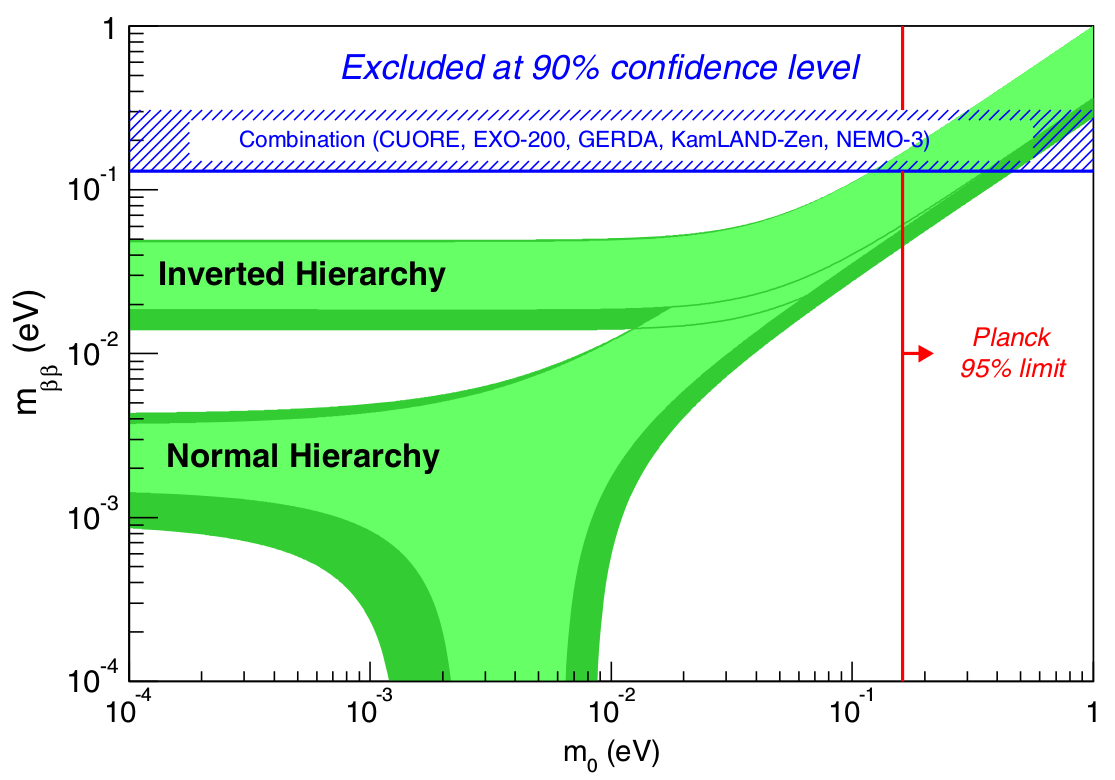
\includegraphics[scale=0.22]{pictures/Chap2/m1NuMassContours2sigma_v4.png}
\caption{Neutrino effective mass for inverted and normal hierarchy with respect to the lightest neutrino mass determined by the best fit oscillation parameters and their uncertainties from~\cite{GlobalFitNeutrinoParameter}. The disfavoured regions from cosmology and 0$\nu\beta\beta$ decay experiments are indicated~\cite{MeffVsM0}.}
\label{EffectiveMassNMM}
\end{center}
\end{figure}


\NI The green bands represent the allowed values of the parameters for m$_{\beta\beta}$ in case of normal and inverted ordering of neutrino mass. The width of each of these bands is mainly governed by the uncertainty over the CP-violating phase. The 0$\nu\beta\beta$ experiments put limits on m$_{\beta\beta}$ (y-axis), while direct and indirect neutrino mass measurements set limits on the lighest neutrino mass (x-axis). The coming 0$\nu\beta\beta$ projects could probe the inverted ordering or excluding 0$\nu\beta\beta$ mediated by the mass mechanism (in case nature chose the inverted ordering). As no neutrinos are emitted, the electrons carry away all the released energy. The total energy distribution of the emitted electrons is expected to be peaked at the Q$_{\beta\beta}$ value as shown in Figure~\ref{EnergySpectrumDBD}. The measurement and the study of the total energy spectrum for the total energy provide the best way to observe 0$\nu\beta\beta$.


\begin{figure}[h!]
\begin{center}
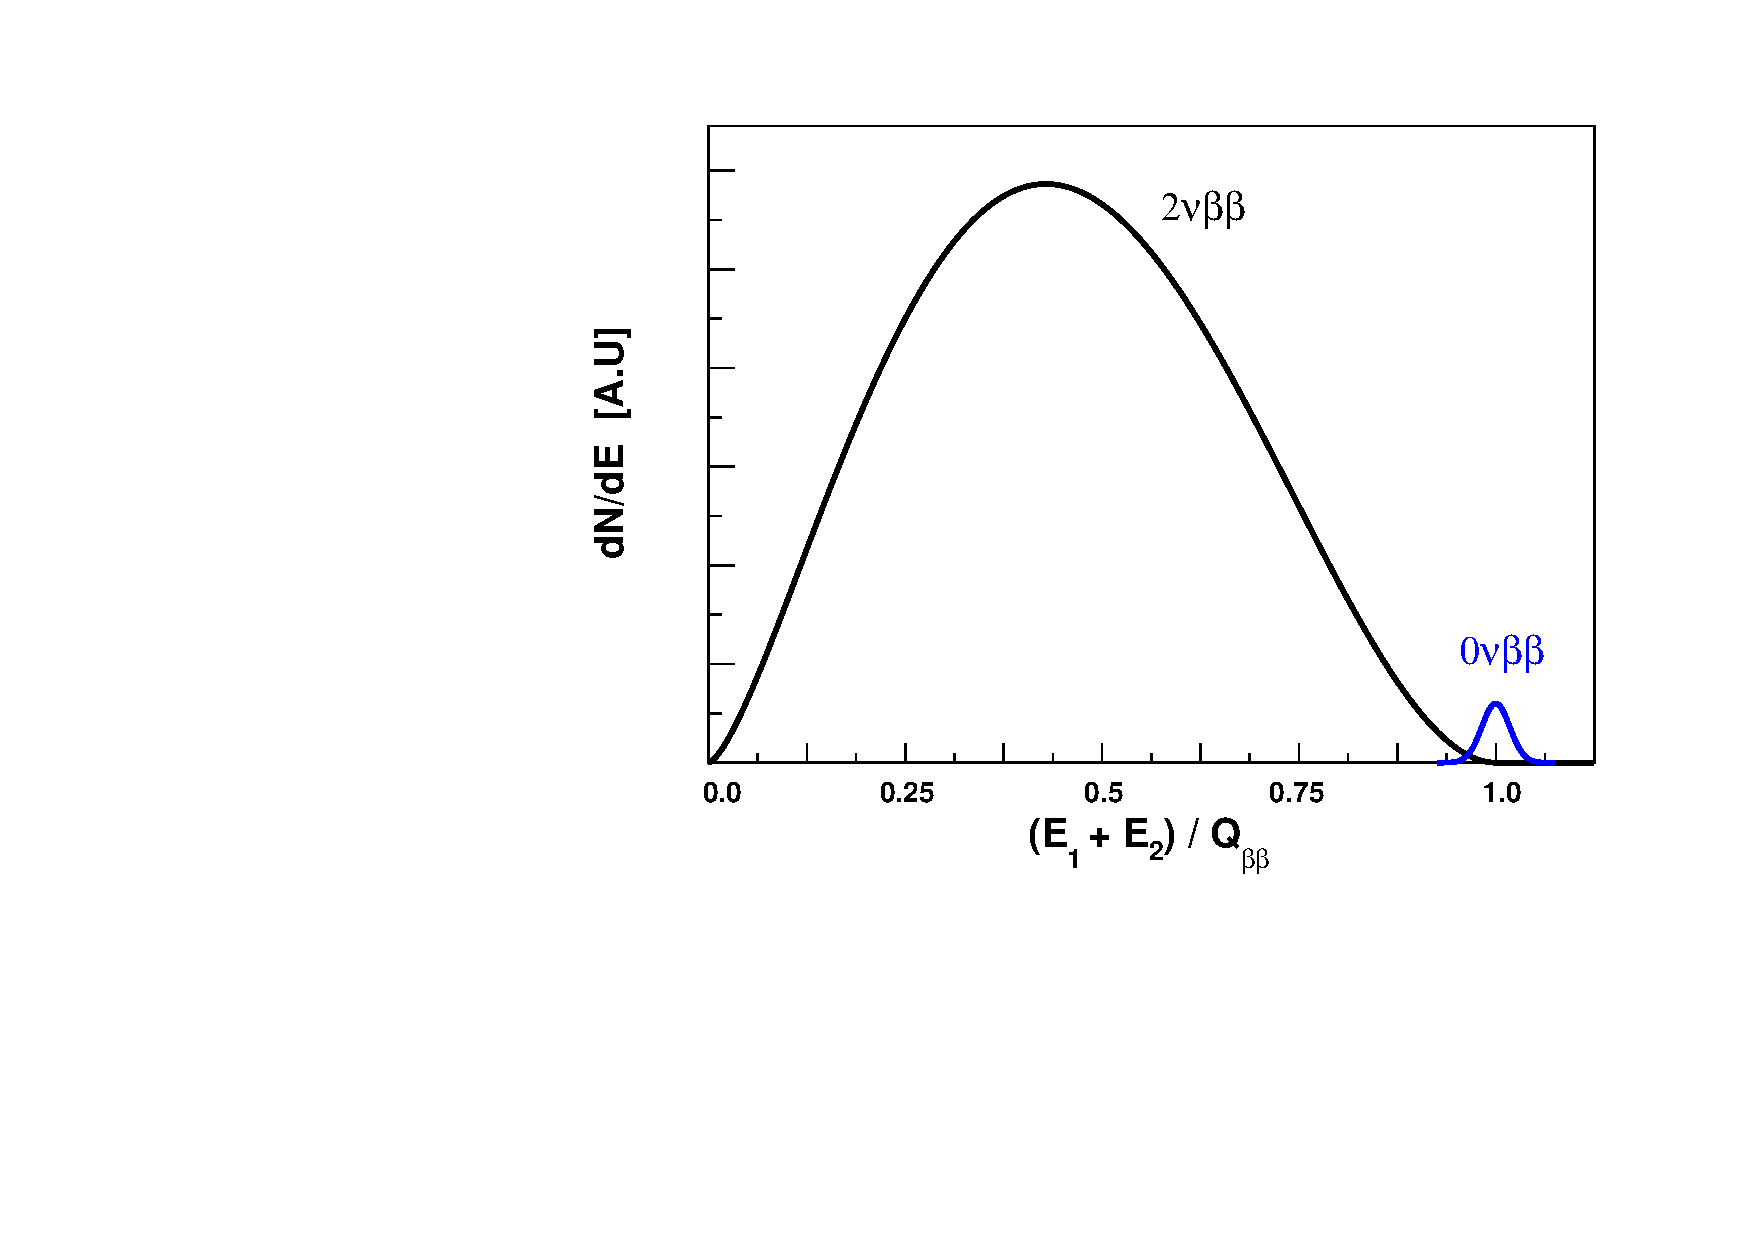
\includegraphics[scale=0.45]{pictures/Chap2/BetaDecaySpectrum.pdf}
\caption{Distribution of the sum of electron energies in case of 2$\nu\beta\beta$ and 0$\nu\beta\beta$. The assumption that $T_{\text{1/2}}^{\text{2}\nu}$ is 1~\% of $T_{\text{1/2}}^{\text{0}\nu}$ has been done.}
\label{EnergySpectrumDBD}
\end{center}
\end{figure}


\FloatBarrier

\subsection{Other mechanisms}\label{sec:OtherMechanisms}


\NI It also exists many other mecanisms which can induce 0$\nu\beta\beta$ decay. All these mechanisms imply new interactions or/and new particles beyond the SM.  The most common and quoted in the literature are the right-handed current and Majoron emission modes. Other processes as R-parity violating super-symmetry, extra dimensions or squark\footnote{superpartner of quark in supersymmetry models} mixing have also been proposed.


%\NI According the considered model, the final topology of the events are different. If one day 0$\nu\beta\beta$ is observed, the measurement of the total energy of the emitted electrons and the angle between them could allow the discrimination between the different mechanisms. Figure~\ref{DifferentbbDecaySpectrum} presented the distribution of total energy electrons according different decays.


\subsubsection{Right-handed Current}


\NI In the SM, all the experimental observations show that parity is maximally violated in weak interactions~\cite{Wu,NeutrinoHelicity}. As a consequence,  only left-handed W boson (W$_\text{L}$) are allowed to interact weakly in the SM. To restore this asymmetry, Left-Right Symmetric models have been proposed and postulate the existence of a new W$_\text{R}$ gauge boson. In these new models V + A vertices are allowed and can lead to 0$\nu\beta\beta$ without a helicity flip. A Feynman diagram for 0$\nu\beta\beta$ decay mediated by right handed current is shown in Figure~\ref{OnbbFeynmanDiagramRHC}, where a W$_\text{L}$ boson couples to a $\bar{\nu}_\text{R}$ at top vertex which is absorbed at the bottom vertex without the need for a helicity change~\cite{DBDRightHandedCurrent}.


\begin{figure}[h!]
\begin{center}
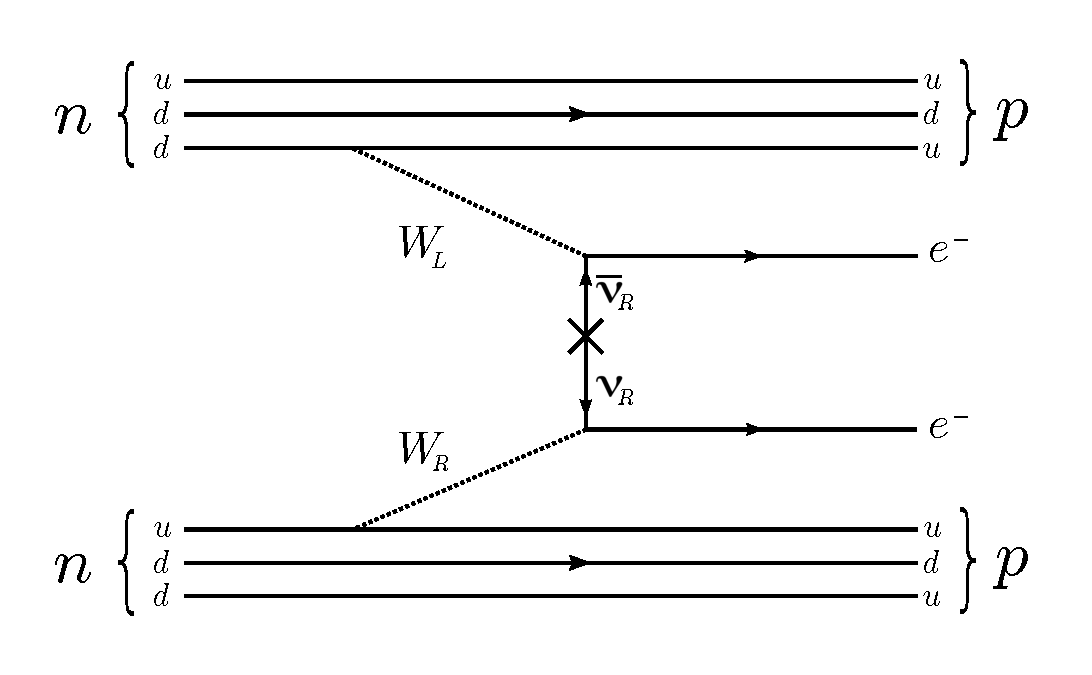
\includegraphics[scale=0.45]{pictures/Chap2/0nubbFeynmanDiagram_RHC.pdf}
\caption{Feynman diagram for 0$\nu\beta\beta$ decay using a right handed current.}
\label{OnbbFeynmanDiagramRHC}
\end{center}
\end{figure}


\bigskip


\NI To describe the physics behind the right handed current two physics parameters are introduced~: $\langle \lambda \rangle$ and $\langle \eta \rangle$. The $\langle \lambda \rangle$ parameter assumes a pure W$_\text{R}$ and describes the coupling between right handed quarks and right handed leptons. In theory, the mediating gauge boson can be a mixture of W$_\text{L}$ and W$_\text{R}$ states. In this case, the $\langle \eta \rangle$ parameter is used to describe the coupling between left handed quarks and right handed leptons and so is related to the mixing angle between W$_\text{L}$ and W$_\text{R}$. These parameters are related to the decay rate as :


\begin{equation}
(\text{T}_{\text{1/2}}^{\text{0}\nu\lambda})^{\text{-1}} = \text{G}_{\text{0}\nu} \times |\text{M}_{\text{0}\nu}|^\text{2} \times \langle \lambda \rangle^\text{2}
\end{equation}

\begin{equation}
(\text{T}_{\text{1/2}}^{\text{0}\nu\eta})^{\text{-1}} = \text{G}_{\text{0}\nu} \times |\text{M}_{\text{0}\nu}|^\text{2} \times \langle \eta \rangle^\text{2}
\end{equation}


\bigskip


\NI As there are two electrons in the final state, the total energy is equal to the Q$_{\beta\beta}$ value of the decay as for the neutrino mass mechanism. To distinguish between the two mechanisms other variables must be used. Due to the presence of the W$_\text{R}$ state at one vertex, the two electrons are preferentially emitted co-linearly which modifies the energy and angular distributions of the electrons as shown in Figure~\ref{TopologyDifferenceNMM-RHC}. These distributions motivate independent measurements for each electron.


\begin{figure}[h!]
\begin{center}
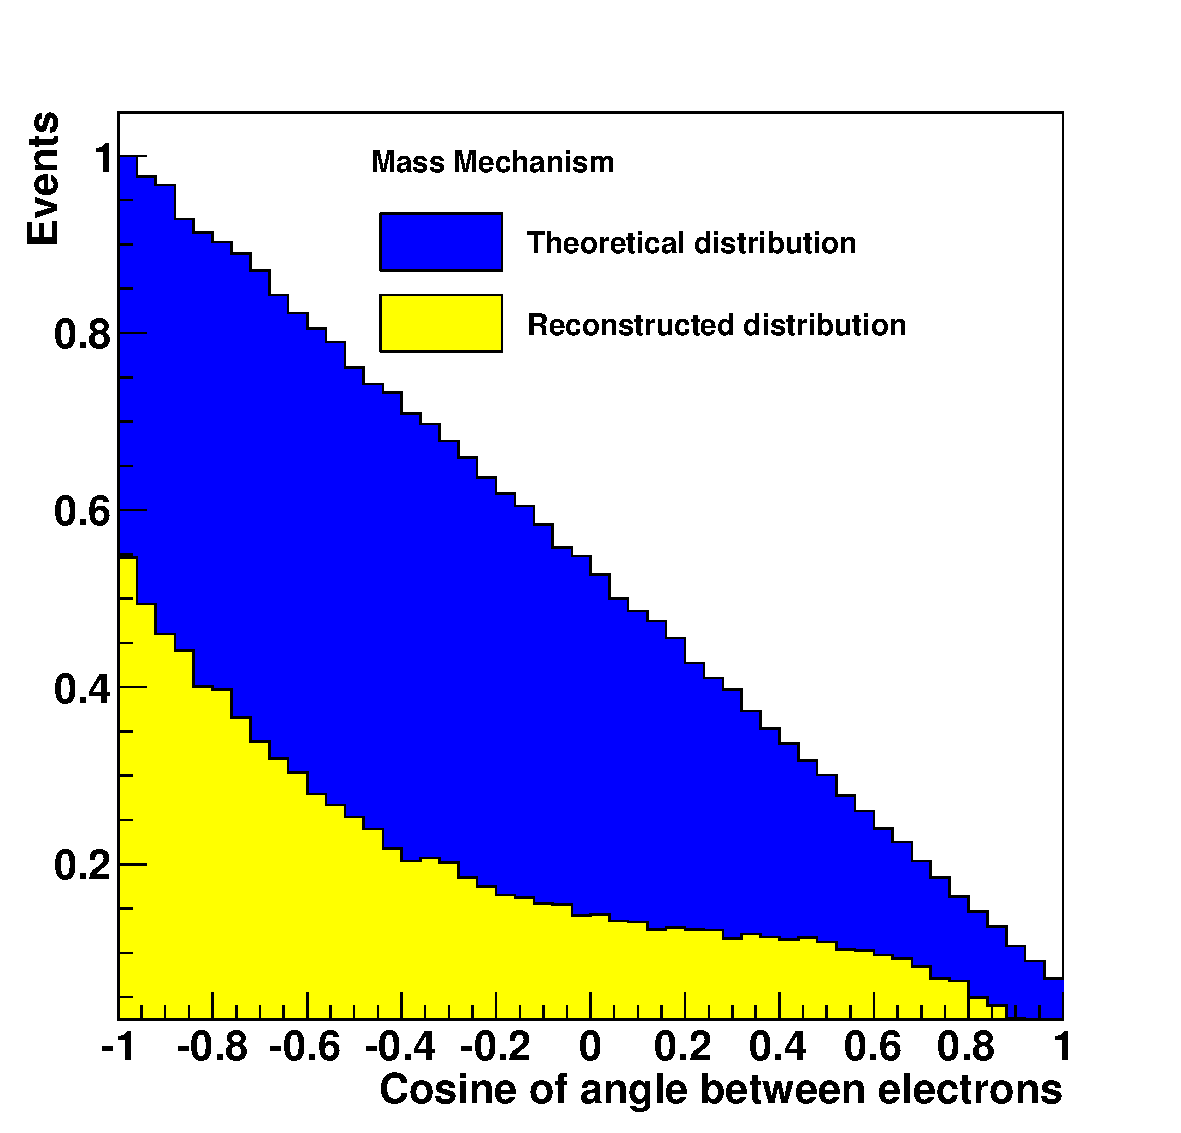
\includegraphics[scale=0.27]{pictures/Chap2/Fig4a.pdf}
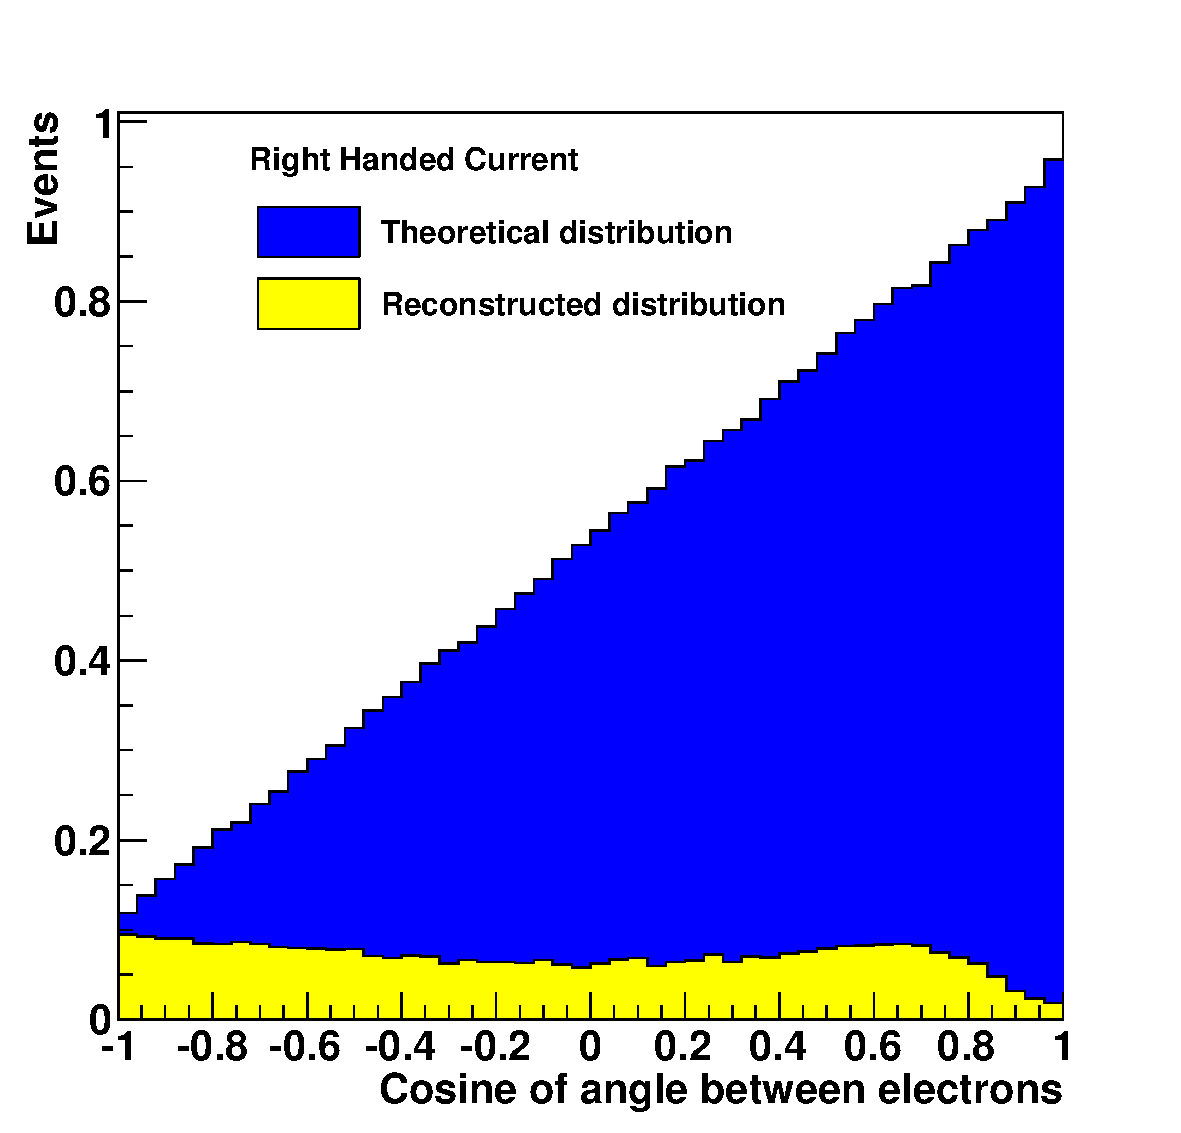
\includegraphics[scale=0.27]{pictures/Chap2/Fig4b.pdf}
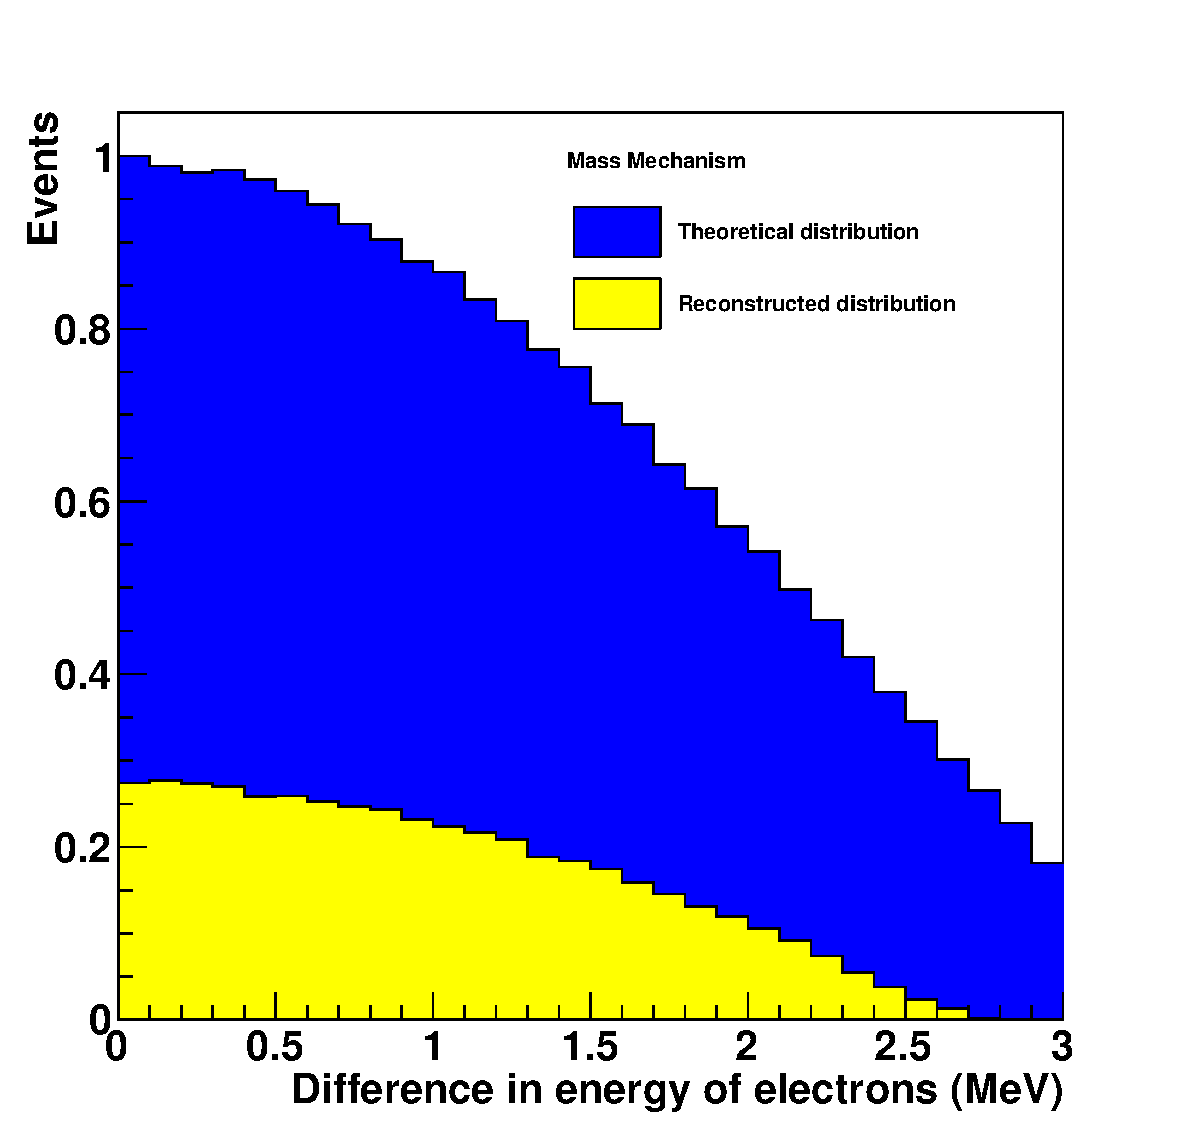
\includegraphics[scale=0.27]{pictures/Chap2/Fig4c.pdf}
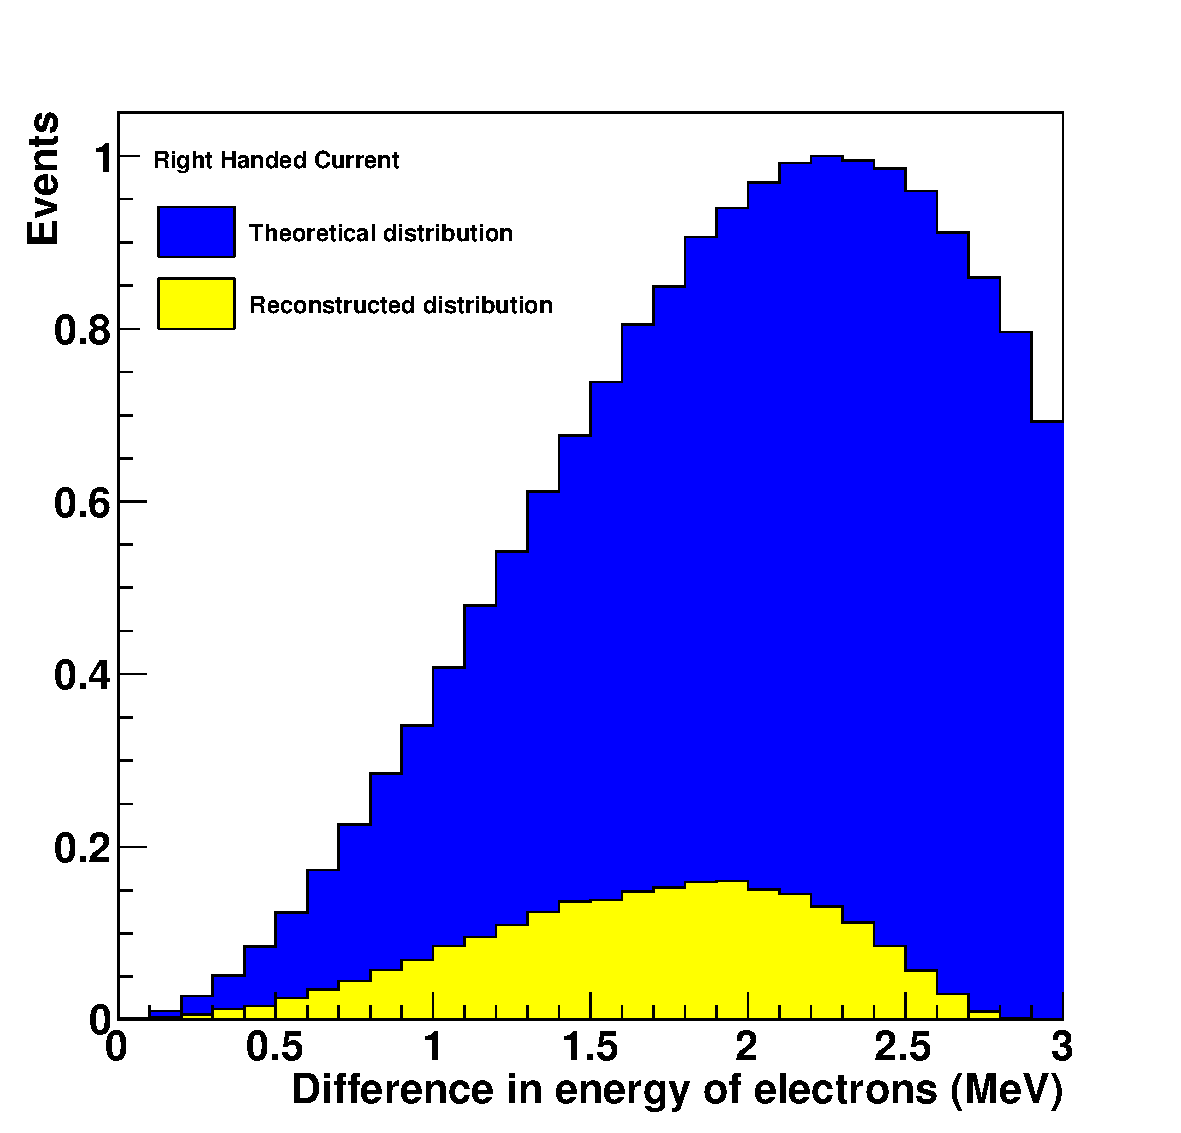
\includegraphics[scale=0.27]{pictures/Chap2/Fig4d.pdf}
\caption{Comparison of the angular and energy difference distribution for the mass mechanism and right-handed current mechanisms. The blue distribution shows the theoretical distrubution while the yellow distribution shows the expected response of SuperNEMO~\cite{ProbingNewPhysicsSN}.}
\label{TopologyDifferenceNMM-RHC}
\end{center}
\end{figure}


\FloatBarrier


\subsubsection{Majoron Emission}


\NI In many theories beyond SM a new global symmetry is introduced relating the difference between baryon and lepton number (B$-$L). In these theories, processes violating individually the baryon number and lepton number are allowed as long as the total quantity B$-$L is preserved~\cite{B-L-Interaction}. Such extensions to the SM require that B$-$L symmetry is spontaneously broken generating a massless Goldstone boson referred to as Majoron ($\chi^\text{0}$) which could provide a mechanism for 0$\nu\beta\beta$. Different models with singlet, doublet and triplet have been developed including couplings to the Z$^\text{0}$ boson~\cite{MajoronEmission1,MajoronEmission2,MajoronEmission3}. Since the doublet and triplet models predict additional coupling to the Z$^\text{0}$ and increase the Z$^\text{0}$ width by the equivalent of half or two extra neutrinos respectively, these models have been excluded by the LEP measurement on the width of the Z$^\text{0}$ boson~\cite{ALEPH3neutrino}. The singlet model is still viable even if it requires an important fine tuning of the neutrino-majoron coupling in order to preserve the current constraints on neutrino mass.


\bigskip


\NI In the 1990s, new models have been proposed to avoid this significant fine tuning. In some of these models the Majoron is massive, carry a lepton number and do not require to be Goldstone boson~\cite{MajoronDecayMode}. They also provide mechanisms leading to 0$\nu\beta\beta$ decay such~as~:


\begin{equation}
\begin{split}
(\text{A},\text{Z}) \rightarrow (\text{A},\text{Z}+\text{2}) + \text{2e}^- + \chi^{\text{0}}~~(\text{singlet}) \\[0.1cm]
(\text{A},\text{Z}) \rightarrow (\text{A},\text{Z}+\text{2}) + \text{2e}^- + \text{2}\chi^{\text{0}}~~(\text{doublet})
\end{split}
\end{equation}


\bigskip


%\NI In these case the half-life of the processes can be written as :


%\begin{equation}
%(\text{T}_{\text{1/2}}^{\text{0}\nu\chi^\text{0}})^{\text{-1}} = \text{G}_{\text{0}\nu\chi^\text{0}} \times |\text{M}_{\text{0}\nu\chi^\text{0}}|^\text{2} \times \langle \text{g}_{\chi^{\text{0}}} \rangle^\text{2}~\text{for}~0\nu\beta\beta\chi_{\text{0}}
%\end{equation}

%\begin{equation}
%(\text{T}_{\text{1/2}}^{\text{0}\nu\chi^\text{0}})^{\text{-1}} = \text{G}_{\text{0}\nu\chi^\text{0}} \times |\text{M}_{\text{0}\nu\chi^\text{0}}|^\text{2} \times \langle \text{g}_{\chi^{\text{0}}} \rangle^\text{4}~\text{for}~0\nu\beta\beta\chi_{\text{0}}\chi_{\text{0}}
%\end{equation}


\NI The Feynman diagrams of two Majoron decays are presented in Figure~\ref{0nubbFeynmanDiagram_Majoron}, the singlet on the left (a) and the doublet on the right (b). In case of doublet, a new hypothetical mediating particle is introduced referred to as zino ($\tilde{\text{Z}}$). This particle comes from the supersymmetry model in which a symmetry between fermions and bosons is predicted~\cite{SUSYbasis}. $\tilde{\text{Z}}$ is the supersymmetric fermion partner to the Z boson.


\begin{figure}[h!]
\begin{center}
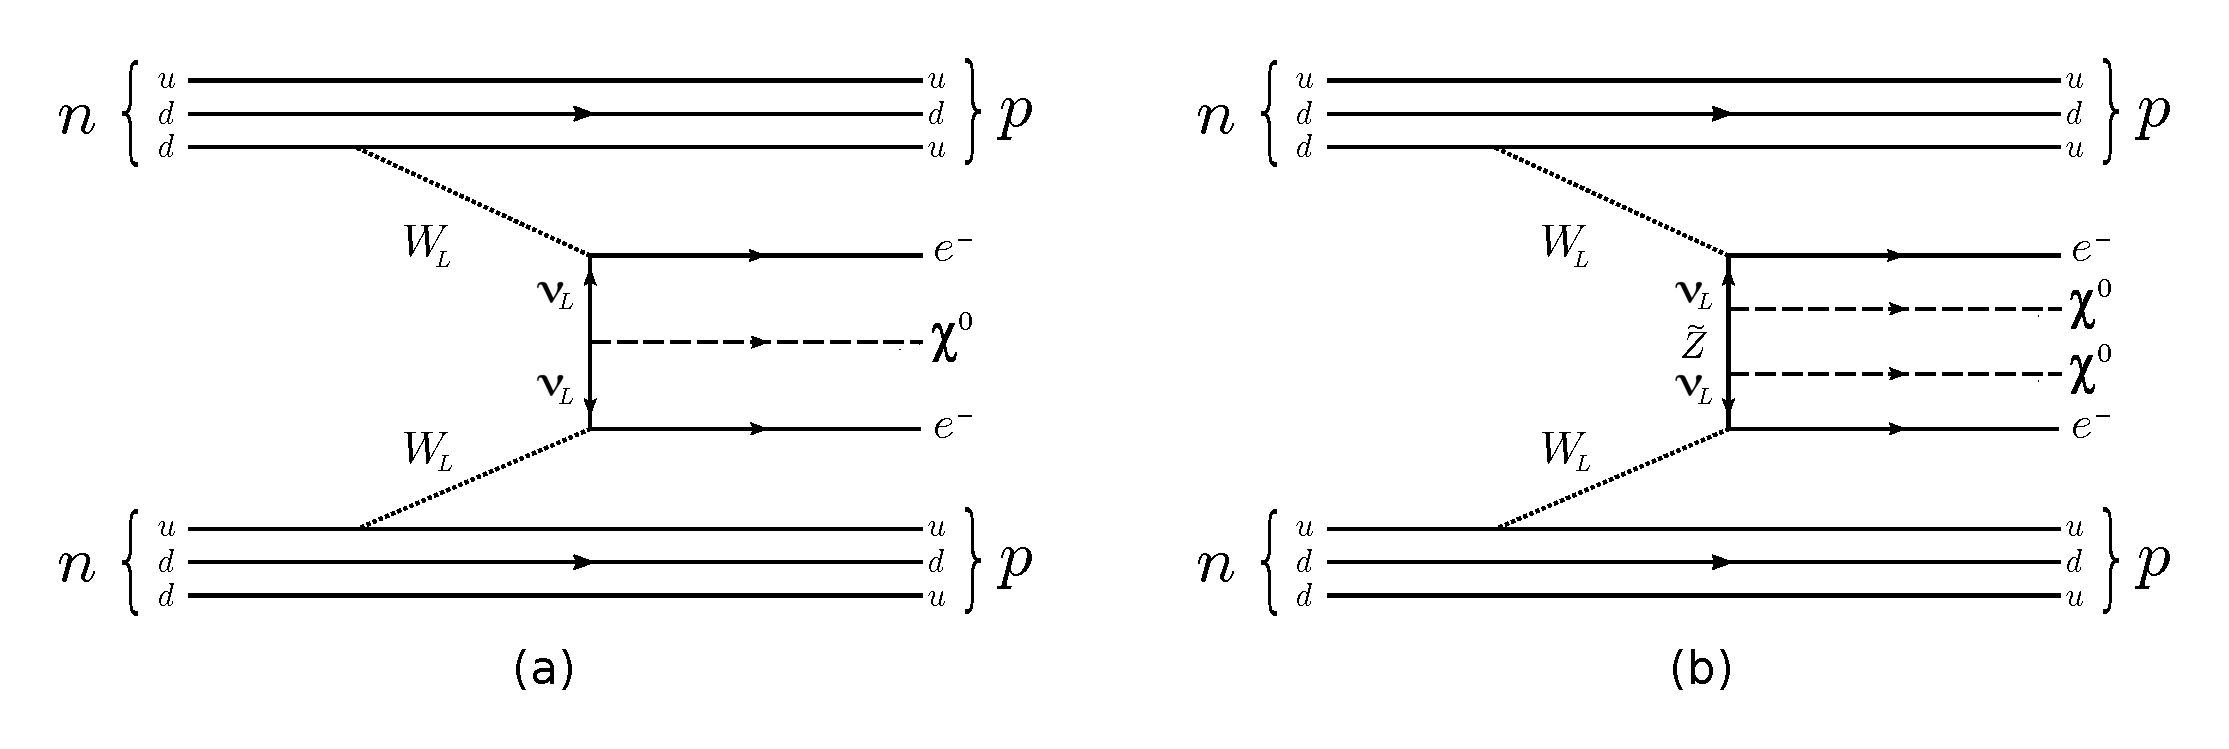
\includegraphics[scale=0.42]{pictures/Chap2/0nubbFeynmanDiagram_Majoron.pdf}
\caption{Feynman diagram for 0$\nu\beta\beta$ decay mediated by Majoron emission with spectral indices $n = 1$ (a) and $n = 2$ (b).}
\label{0nubbFeynmanDiagram_Majoron}
\end{center}
\end{figure}


\NI Ten different Majoron models exists which can provide a mechanism for 0$\nu\beta\beta$ decays~\cite{MajoronDecayMode}. Some of them conserve the lepton number while others violate it. To differentiate between these models the total energy of the electrons can be used. As extra particles are emitted the energy spectrum is not a monochromatic line but a continuous spectrum. The shape of this spectrum is affected in different ways according to the Majoron model. This spectrum modification is governed by the spectal index, n, describing the dependance of the phase space factor on the Majoron(s) energy : 


\begin{equation}
\text{G}_{\text{0}\nu\chi^\text{0}} \propto (\text{Q}_{\beta\beta} - \text{E}_{\text{e1}} - \text{E}_{\text{e2}})^\text{n}
\end{equation}


\NI where E$_{\text{e1}}$ and E$_{\text{e2}}$ are the energy of the emitted electrons, Q$_{\beta\beta}$ the nuclear transition energy and G$_{\text{0}\nu\chi^\text{0}}$ the space phase factor. The electron energy distribution for n equal 1, 2, 3 and 7 are given in Figure~\ref{DifferentbbDecaySpectrum}.


\bigskip


\begin{figure}[h!]
\begin{center}
%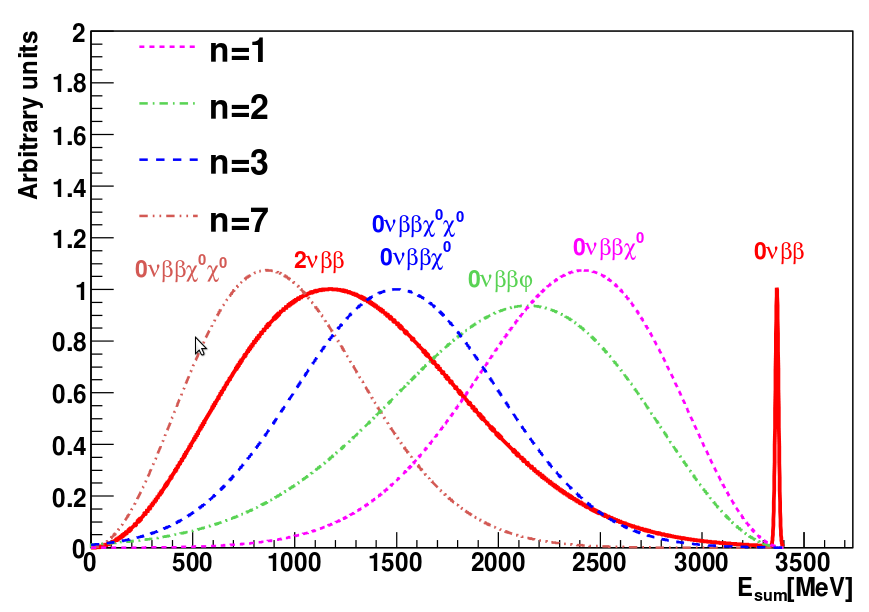
\includegraphics[scale=0.35]{pictures/Chap2/MultipleMajoronEmissionElectronEnergySpectrum.png}
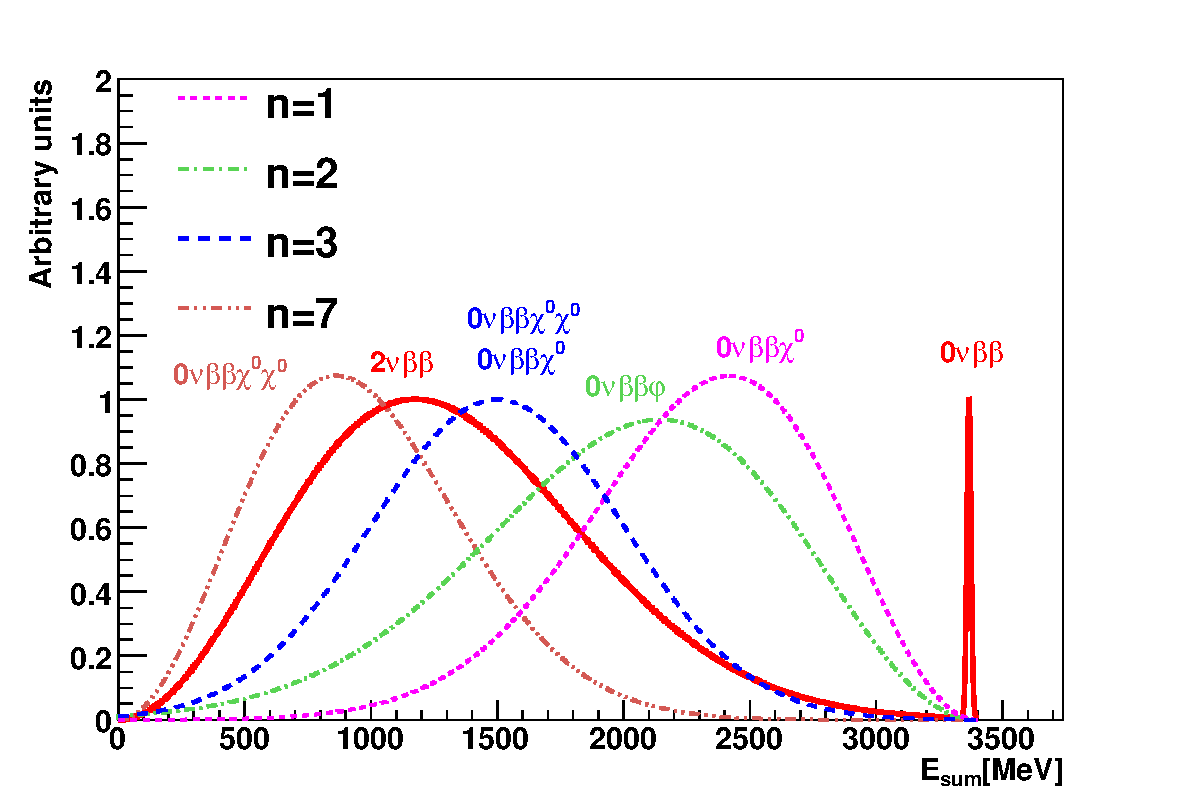
\includegraphics[scale=0.5]{pictures/Chap2/esum_theory.pdf}
\caption{Distribution of the sum of electron energies for 2$\nu\beta\beta$ and 0$\nu\beta\beta$ according to different Majoron decay modes with spectal indices 1,2,3 and 7 \cite{FatemiGhomiThesis}.}
\label{DifferentbbDecaySpectrum}
\end{center}
\end{figure}


\FloatBarrier


\subsection{Nuclear Matrix Element}\label{sec:NME}


\NI In order to set a value or a limit on the physics parameter $\eta$ of the Equation~\ref{eq:halflife0nu} from the experimentally measured T$_{\text{1/2}}^{\text{0}\nu}$, the phase space factor and the nuclear matrix element (NME) must be evaluated. The phase space factors which include the kinematics of the decay can be calculated with good precision. Due to the many-body nature of the problem, the computations of the NME are not trivial and different assumptions have to be made to facilitate them which led to the developement of different models.  The NME of the 0$\nu\beta\beta$ decay can be expressed as :

%This can be even more complicated as the ground state and many different excited states of open-shell nuclei with complated nuclear structures must be considered~\cite{TheoryOfNeutrinolessDBD}.

\begin{equation}
|\text{M}_{0\nu}| = |\text{M}_{\text{GT}}^{0\nu} - \frac{\text{g}_{\text{Av}}^\text{2}}{\text{g}_\text{V}^\text{2}} \text{M}_\text{F}^{0\nu} + \text{M}_\text{T}^{0\nu}|
\end{equation}


\bigskip


\NI where g$_{\text{Av}}$ and g$_\text{V}$ are the axial-vector and vector coupling constants of the weak interaction and M$_{\text{GT}}^{0\nu}$, M$_{\text{F}}^{0\nu}$ and M$_{\text{T}}^{0\nu}$ are the Gamov-Teller, Fermi and tensor parts of the NME. M$_{\text{T}}^{0\nu}$ is neglected in most of the calculations due to its small contribution.


\bigskip


\NI All the methods which have been implemented for the calculation of NME involve two different stages. In a first step, the interactions between nucleons, the nuclear physics informations and the physical mechanism behind 0$\nu\beta\beta$ are incorporated via a many-body Hamiltonian. The second step consists in an introduction of a mean field to take into account the nuclear structure and residual interactions. It is in this second step that the models tend to differ by introducing different approximations and/or simplifying assumptions. This section briefly describes the different models and the difference between them. %A comparison of the NME calculation results are given in the last section. 


\subsubsection{Interacting shell model}


\NI The interacting shell model (ISM) handles a limited number of nuclear orbitals close to the Fermi level\footnote{The Fermi level is a thermodynamic quantity corresponding to the total chemical potential for the electrons. Its meaning is the thermodynamic work required to add one electron to the body.}~\cite{ISM_1,ISM_2,ISM_3,ISM_4}. This model considers all the possible correlations between nucleons, proton-proton, neutron-neutron and proton-neutron, such that both proton and neutron numbers are conserved. It is accepted that this model works well for light nuclei such as $^{\text{48}}$Ca, $^{\text{76}}$Ge and $^{\text{82}}$Se but is not appropriate for calculations involving heavy or deformed nuclei such as $^{\text{150}}$Nd where orbitals far from the Fermi level must be taken into account.


\subsubsection{Quasiparticle random phase approximation}


\NI Contrary to ISM, the quasiparticle random phase approximation model (QRPA) considers a high number of nuclear orbitals with reduced interactions between the nucleons~\cite{QRPA_1,QRPA_2,QRPA_3}. The NME are calculated by assuming that the initial and final nuclear states are connected via many virtual intermediate collective states. As the proton-proton and neutron-neutron interactions are treated separately the proton and neutron numbers are not nececessarily conserved in this model. It is accepted that the QRPA model gives more reliable results for heavy nuclei but this model can also be used to compute NME of lighter nuclei. Deformations in the initial and final state wave functions can be introduced in the calculations. 


\subsubsection{Interacting boson model}


\NI The interacting boson model (IBM) is a model in which protons and neutrons pair up and act as a single particle having boson properties~\cite{IBM}. Two versions of the model exist depending if protons and neutrons are treated in the same way (IBM-1) or separately (IBM-2). Due to the pairing, only the even-even nuclei are taken into account by the IBM model, which is not a problem since only even-even nuclei can undergo 0$\nu\beta\beta$ decay as seen before. The IBM is, in form, quite similar to ISM.


\subsubsection{Other methods}


\NI Other methods exist to compute the NME such as projected Hartree-Fock-Bogoliubov (PHFB)~\cite{PHFB_1,PHFB_2} and energy density function (EDF)~\cite{EDF_1,EDF_2,EDF_3}. The PHFB method has been successful in the study of 2$\nu\beta\beta$ but may suffer from a certain degree of oversimplification. The EDF method is an improvement of the PHFB method which takes into account the inter-nucleon interactions.


\subsubsection{Comparison of the NME calculations}


\NI In order to understand the consequences of the assumptions made by the different models it is interesting to compare the NME results given by each method. This comparison has to be done carefully since different values are used in the calculations. Mostly for historical reasons, the ratio of the vector and axial-vector couplings, g$_{\text{A}}$, is set at either 1.0 or 1.25. Moreover, the value which parameterizes the size of the atomic radius, r$_0$ is either 1.1~fm or 1.2~fm~\footnote{The atomic radius R$_\text{A}$ is commonly parametrised as r$_0$A$^{\text{1/3}}$~\cite{RadiusNucleus}}. The results of the NME calculations with the values g$_{\text{A}}$~=~1.25 and r$_0$~=~1.2~fm are shown in Figure~\ref{NME}. The results obtained by Tübingen-Brastislava-Caltech and Jyväskylä groups using QRPA method are referred to as QRPA~(T) and QRPA~(J) respectively. Depending on the isotopes, the results differ to factor of 2-3. The ISM method tends to overestimate the correlations between the nuclear orbitals reducing the values of the NME and making the nucleus more stable. 


\bigskip


\NI Except for the ISM model, the results for $^{\text{130}}$Te and $^{\text{136}}$Xe are in good agreement. Moreover the QRPA~(T) and IBM methods agree across all isotopes. The disparities between the two QRPA methods, and more particularly for $^{\text{82}}$Se, $^{\text{96}}$Zr and $^{\text{100}}$Mo are still unexplained. 


\bigskip


\NI It is not possible to measure M$^{0\nu}$  independently from measuring the 0$\nu\beta\beta$ half-life. The large range of M$^{0\nu}$ translates into a large uncertainty on the limits for 0$\nu\beta\beta$ processes. Different ways are explored to succeed in reducing uncertainties. Recently, thanks to the measurements of $\beta$ and $\beta\beta$-decay half-lives for different isotopes, QRPA calculations of M$_{\text{GT}}^{0\nu}$ can be more constrained leading to a reduction of the M$^{0\nu}$ uncertainties. Moreover, the different models used to compute the NME values are also used to predict some observables of nuclear structure such as valence nucleon occupencies or nucleon paring correlations. A dedicated program has been created to measure these observables in order to compare them with the theoretical predictions~\cite{ReduceNMEuncertainties}. These results could aslo be used to tune the models. Finally, the decay via the excited state of the daugher nucleus can bring additional informations on the nuclear structure and help for the NME calculations. 


\begin{figure}[h!]
\begin{center}
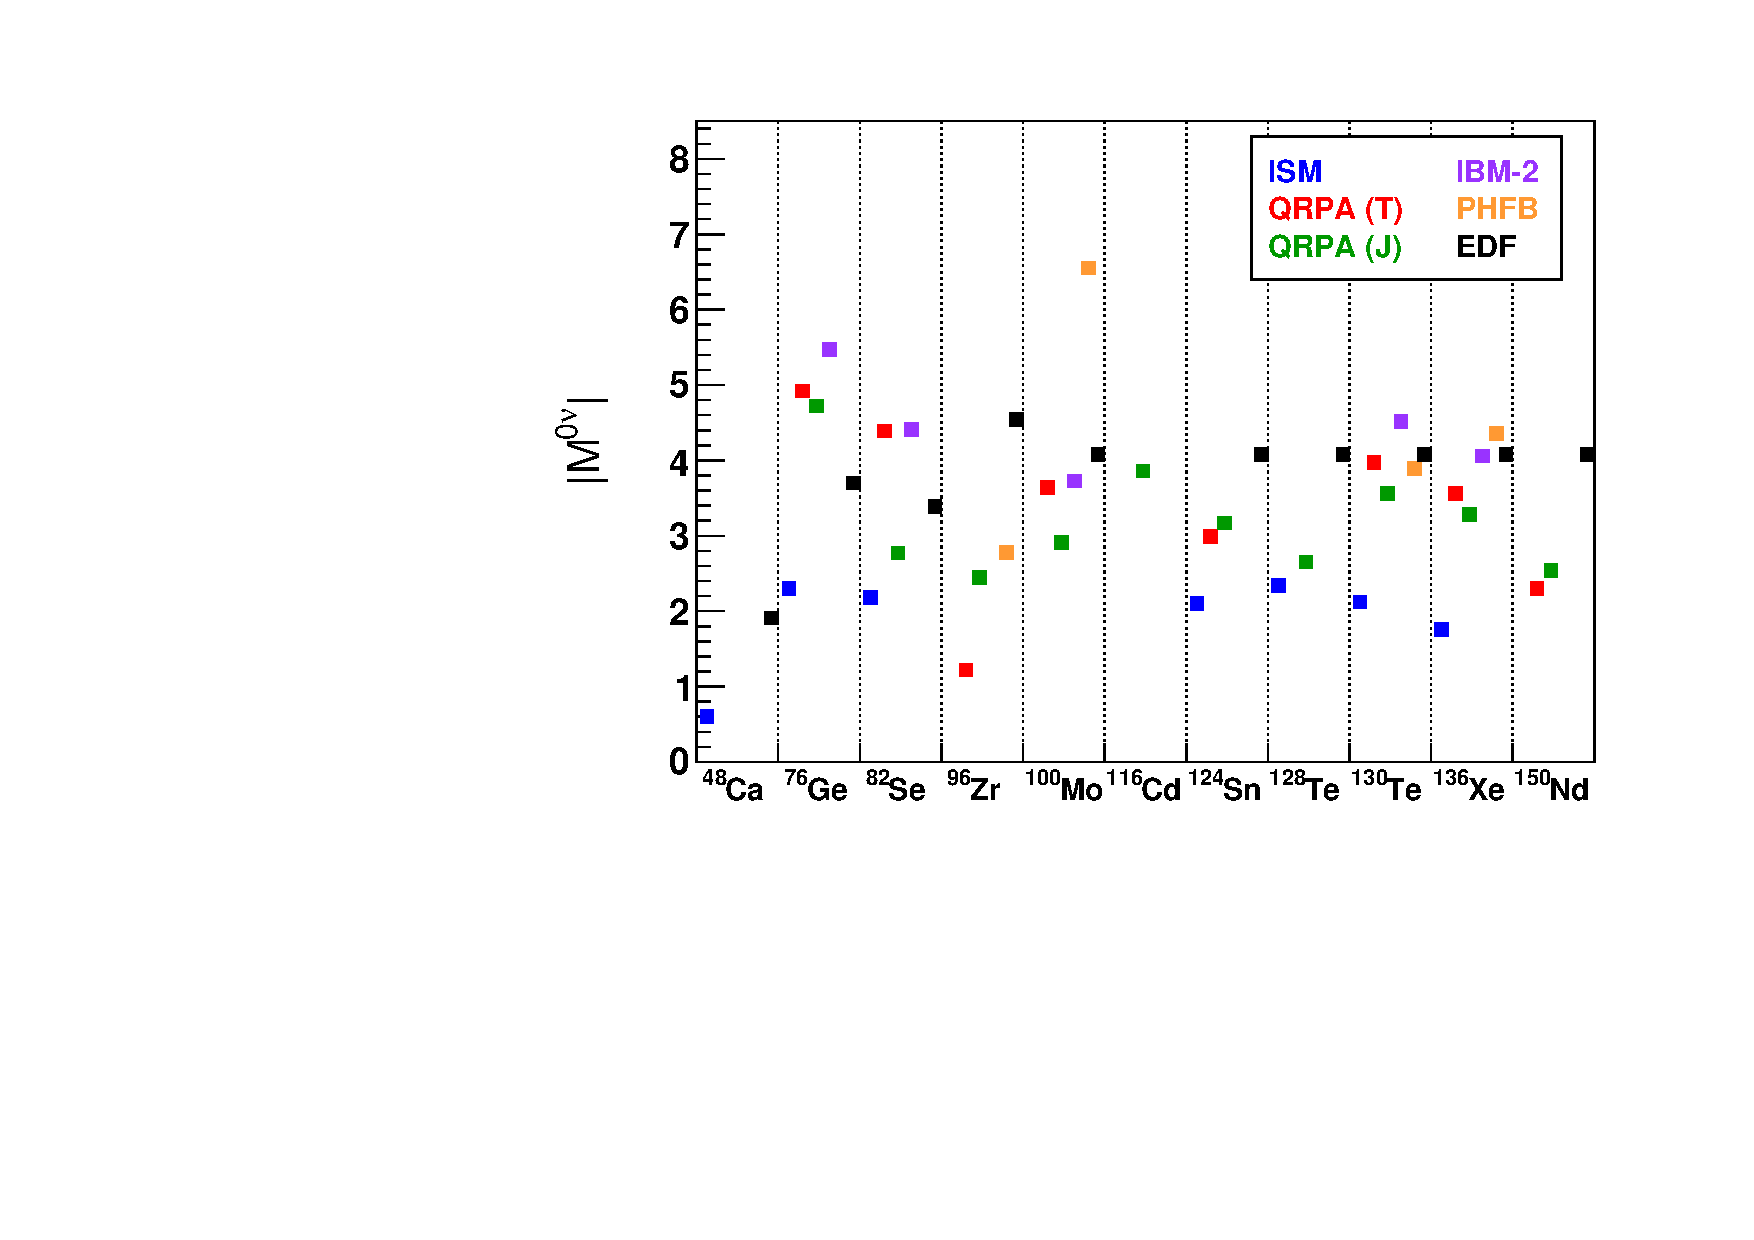
\includegraphics[scale=0.6]{pictures/Chap2/NMEvalue.pdf}
\caption{Summary of 0$\nu\beta\beta$ Nuclear Matrix Element (NME) computations, calculated for 11 isotopes, using different approaches. These results are extracted from \cite{TheoryOfNeutrinolessDBD}, conversion for g$_{\text{A}}$ = 1.25 and r$_{\text{0}}$  = 1.2~fm have been made when necessary.}
\label{NME}
\end{center}
\end{figure}


\FloatBarrier


\section{Experimental search for $\beta\beta$ decays}\label{sec:ExperimentalSearch0nu}


\NI Despite that the 2$\nu\beta\beta$ decay is very rare and very challenging to observe, their observation is a confirmation of the SM at the second order which provides additional information on the nuclear structure. Concerning the 0$\nu\beta\beta$ decay its detection would confirm the Majorana nature of the neutrino and could give access to their mass scale. It is for these reasons that many experiments searching for $\beta\beta$~decays have been built around the world. This section presents the general considerations to design a $\beta\beta$ experiment in order to reach the best sensitivity on the $\beta\beta$ processes.


\subsection{Half-life sensitivity for 0$\nu\beta\beta$}


\NI The expected half-life sensitivity that an experiment can reach for the 0$\nu\beta\beta$ decay can be approximately pramametrised with the following expression~\cite{formulaSensBB} : 


\begin{equation}\label{eq:sensitivity0nu}
\text{T}_{\text{1/2}}^{0\nu} (\text{n}_\sigma) = \frac{\text{4.16}~\times~\text{10}^{\text{26}}~\text{y}}{\text{n}_\sigma} \left(\frac{\epsilon \text{a}}{\text{W}} \right) \sqrt{\frac{\text{MT}}{\text{b}\Delta\text{E}}}
\end{equation}


\bigskip


\NI where T$_{\text{1/2}}^{0\nu}$ is the half-life sensitivity to 0$\nu\beta\beta$ in years, n$_\sigma$ is the number of standard deviations for a given confidence level (90\% CL corresponds to n$_\sigma$~=~1.64), $\epsilon$ is the detection and identification efficiency, a is the isotopic abundance of the 0$\nu\beta\beta$ source isotope of the source mass, W is the weight of the source isotope, M is the total mass of the source in [kg], T is the live time of the experiment in [y], b is the background rate in [keV kg y]$^{-\text{1}}$, and $\Delta$E is the energy resolution in [keV] at the Q$_{\beta\beta}$ value of the isotope. 


\bigskip


\NI Equation~\ref{eq:sensitivity0nu} demonstrates that to obtain the best sensitivity value, an experiment has to investigate a huge amount of isotope mass during the longest possible time with a very good detection efficiency, a very good energy resolution and with the lowest background possible. Generally, to maximise the sensitivity of an experiment, the highest signal efficiency and the lowest level of background is seeked.


\subsection{Maximising signal}


\NI To maximise the chance to observe a $\beta\beta$ decay, an experiment should study a large number of atoms of isotopes for as long as possible. Futhermore, even if a decay occurs, the detector must not miss it, thus the experiment must have a high effiency detection to maximise the sensitivity.


\bigskip

\NI The choice of the $\beta\beta$ isotope is also important when looking to maximise the signal. Indeed, as shown in Eq.~\ref{eq:decayRate2nu} and~\ref{eq:halflife0nu} the phase space factors and the NME are related with the decay rate. Isotopes with high phase space factor and NME have a shorter half-live compared to the others. As a result, in the same amount of time, more decays can occur, which makes their detection more likely. 


\bigskip


\NI The molar mass of the isotope also plays a role in the maximization of the signal since it influences the total number of atoms in the sample. This parameter is generally not considered since there is a factor around 5 between the lighter and the heavier  isotopes ($^{\text{46}}$Ca and $^{\text{238}}$U) which is neglectable compared to the G$^{\text{0}\nu}$ which can variates over a factor around 2.10$^{\text{4}}$ depending on the isotpe ($^{\text{80}}$Se and $^{\text{150}}$Nd). 


\bigskip


\NI The natural abundance and the ability to enrich an isotope must be taken into consideration. To reach a considerable mass of $\beta\beta$ isotope, it is simpler and cheaper if the isotope is already present in large quantities in nature. Depending on the isotope, different enrichment techniques exist having different yields and prices. The majority of the isotopes can be enriched via centrifugation method which is relatively cheap and allows the enrichment up to large mass. For some isotopes, such as $^{\text{48}}$Ca, only electromagnetic separation is available, which only allows the enrichment of smaller quantities.


\subsection{Minimising background}\label{sec:MinimisingBkg}


\NI By looking at the Equation~\ref{eq:sensitivity0nu} which assumes a gaussian background it makes sense that an ideal 0$\nu\beta\beta$ experiment should minimize the b$\times\Delta$E term to increase the half-life sensitivity. As seen before, $\beta\beta$ decays is a very rare process, in which two electrons are emitted with a typical energy of a few MeV (2.0 - 4.3~MeV depending on the isotope). The main background in the search for $\beta\beta$ decay is the natural radioactivity in which particles with similar energy are emitted. The two main isotopes to the background are the radioactive elements $^{\text{214}}$Bi and $^{\text{208}}$Tl, which are naturally present in small quantities in the materials from the $^{\text{238}}$U and $^{\text{232}}$Th decay chains shown in Figure~\ref{u238-th232decayChain}. The electrons and photons emitted during the decays can by different processes such as Bremsstrahlung, Compton or Möller scatterings mimic the 2e signal. To suppress this background, the detector materials must be carefully chosen to be radiopure. Futhermore, to reduce the $^{\text{214}}$Bi and $^{\text{208}}$Tl contributions, it is preferable to select a $\beta\beta$ isotope with a high Q$_{\beta\beta}$ value to get away from the natural radioactivity, the highest energy $\gamma$-ray in the decay chain of $^{\text{238}}$U and $^{\text{232}}$Th is emitted by $^{\text{208}}$Tl at 2.6~MeV.


\bigskip  

%\NI In the scenario of a background-free experiment, this equation becomes linear, explaining why it is important to reduce the background :

%begin{equation}
%\text{T}_{\text{1/2}}^{0\nu} (\text{n}_\sigma) = \frac{\text{4.16}~\times~\text{10}^{\text{26}}~\text{y}}{\text{n}_\sigma} \left(\frac{\epsilon \text{a}}{\text{W}} \right) \times \text{MT}
%\end{equation}

%\NI As seen before, $\beta\beta$ decays is a very rare process, in which two electrons are emitted with a typical energy of a few MeV (2.0 - 4.3 MeV depending on the isotope). The main background in the search for $\beta\beta$ decay is the natural radioactivity in which particles with similar energy are emitted. 


\NI Another source of background comes from cosmic rays. To reduce it, the experiments are placed in an underground laboratory where the muon flux is highly suppressed. Futhermore, shieldings are generally used to protect the detector from the neutrons coming from muon spallation on nuclei and natural radioactivity of the surrounding laboratory rocks.


\bigskip


\NI Some detectors have the ability to reconstruct the full event topology,  which coupled with analysis techniques can be used to differentiate the signal from the background events and highly suppress the background.


\bigskip


\NI The tail of the 2$\nu\beta\beta$ process constitutes an irreducible background to the search for the 0$\nu\beta\beta$. Indeed, the 0$\nu\beta\beta$ signal is expected to be mono-energetic located at the end-point of the spectrum but due to the limited energy resolution of the detector an overlap with the 2$\nu\beta\beta$ event can occurs. This background can only be suppressed by improving energy resolution of the detector.  


\begin{figure}[h!]
\begin{center}
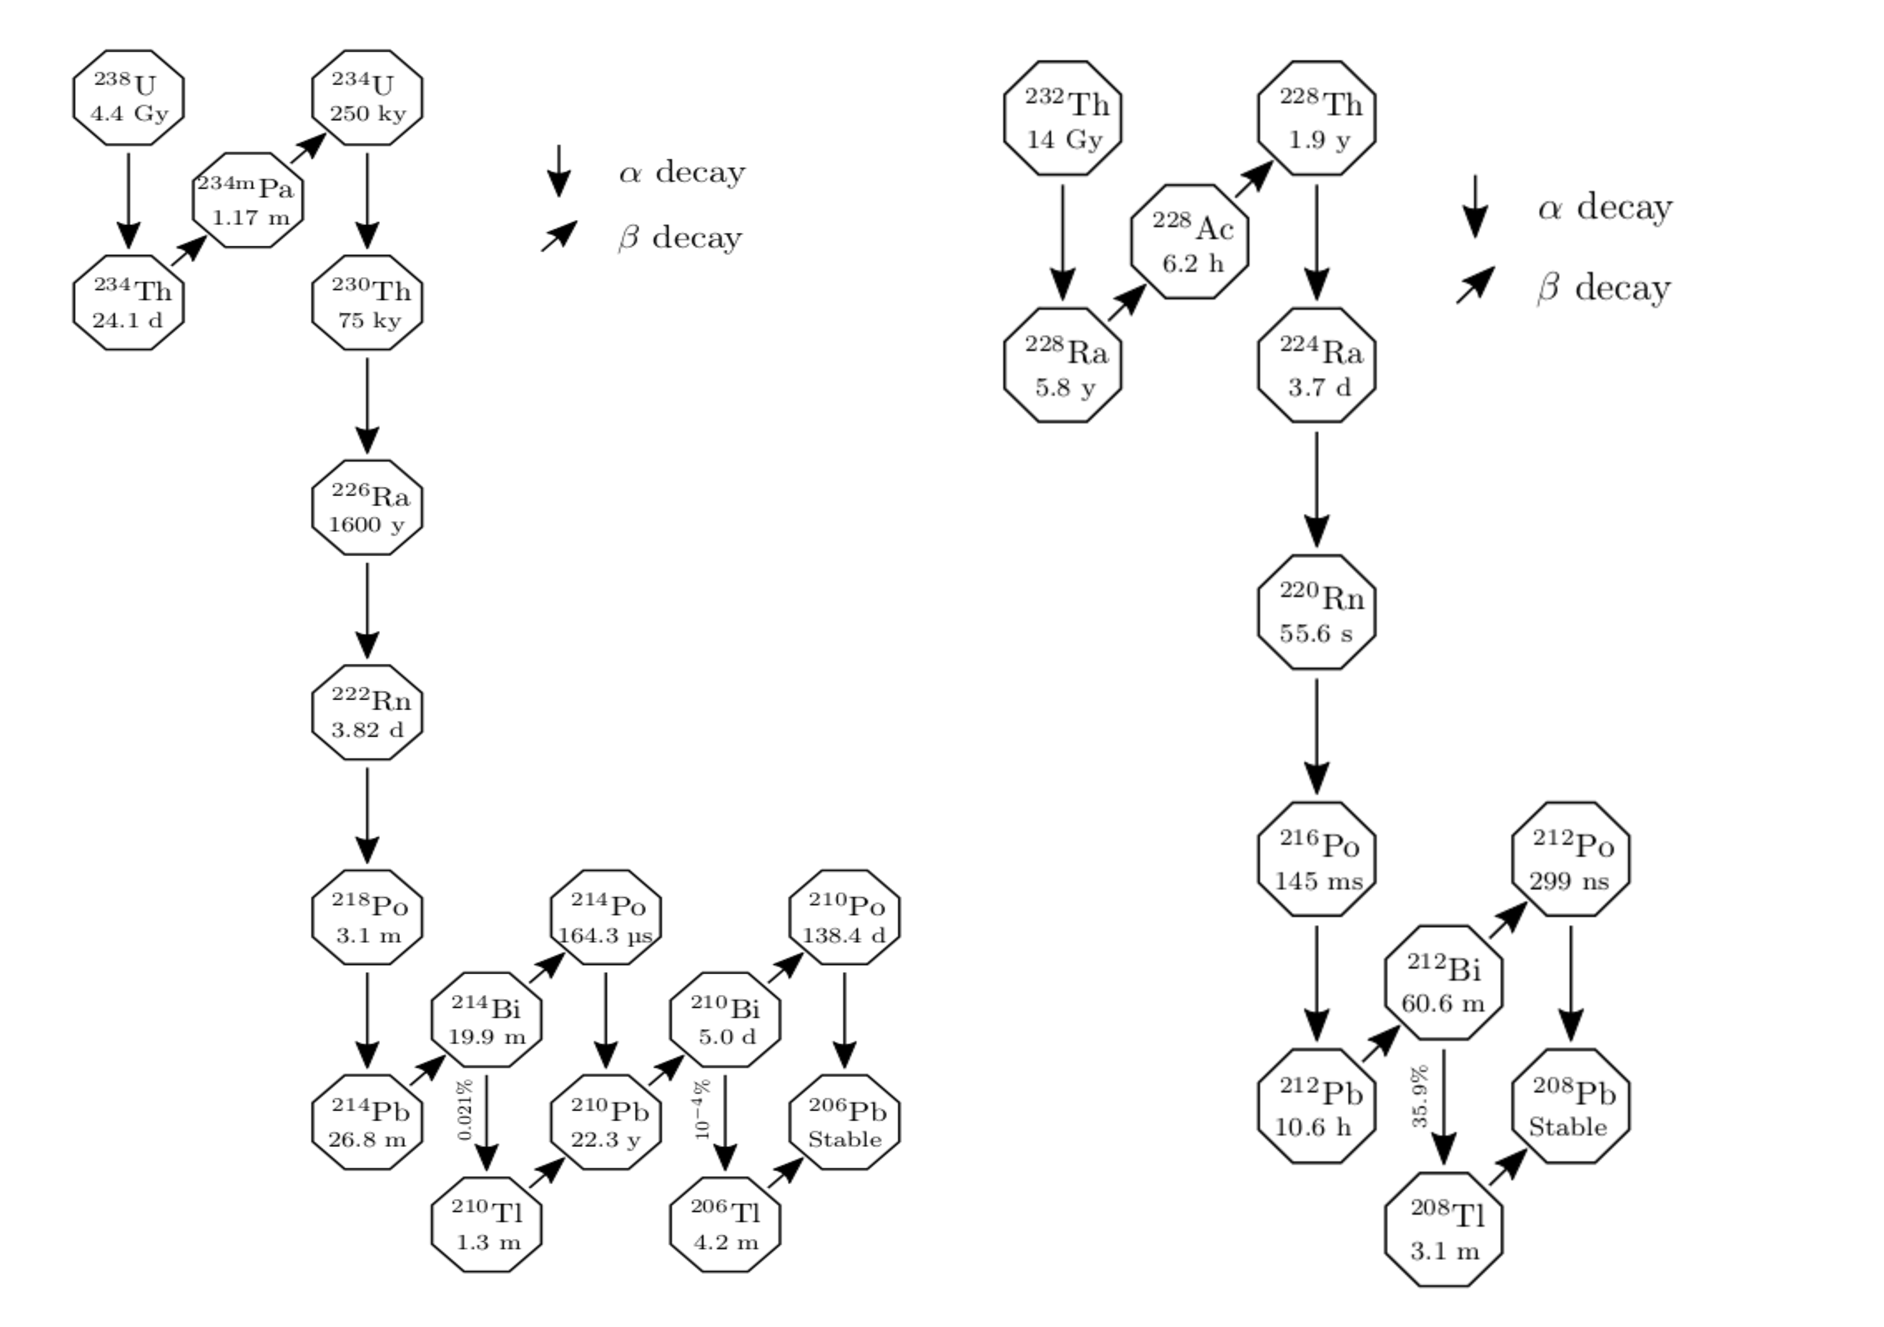
\includegraphics[scale=0.40]{pictures/Chap2/u238-th232decayChain.pdf}
\caption{Left : $^{238}$U decay chain, the downward arrows represent the $\alpha$ decay and the upward arrows represent the $\beta$ decay. The same element is shown on horizontal lines. If an isotope can decay in multiple modes, the branching ratios are written on the $\alpha$ transition. Right : $^{232}$Th decay chain.}
\label{u238-th232decayChain}
\end{center}
\end{figure}


\FloatBarrier


\section{Double Beta Experiments}\label{sec:DBDexperiment}


\NI To design a $\beta\beta$ experiment, several factors must be taken into account as demonstrated in Equation~\ref{eq:halflife0nu}. Unfortunately some of these factors are inversely related to each other, such as favoring one can deteriorate the others. For example, building an experiment with a huge amount of $\beta\beta$ isotope is not possible without also increasing the level of background. As a result, many experiments have been developed in order to optimize the sensitivity to 0$\nu\beta\beta$ decay in different ways. This section presents the different experiments with their advantages and disadvantages. A summary of recent results of each experiment is also given.


\subsection{Semiconductor experiments}


\NI Some semiconductors such as germanium have some isotopes which undergoes $\beta\beta$ decays, and can be used both as $\beta\beta$ decay source and detector. The $\beta\beta$ isotope, usually~$^{\text{76}}$Ge, is placed between two electrodes. Ionizing radiation creates electron-hole pairs in the material. The electrons are drifted towards the electrodes and produce signals which are proportional to the total energy of the decay. Due to their homogeneous design, semiconductor experiments have a very high acceptance and detection efficiency. These detectors typically work at cryogenic temperatures, to suppress the electronic noise. This has also the advantage of obtaining a very good energy resolution, $\sim$~0.3~\% FWHM at the Q$_{\beta\beta}$ value of $^{\text{76}}$Ge~\cite{QbetabetaGe}. %By using the segmentation of the semiconductors and by analysing the electrode pulse shapes some background events can be removed. 
These detectors have only access to the total energy deposit and can not measure the full topology of the two electrons being emitted. Five old and recent semiconductor experiments are decribed in the following section.


\subsubsection{Heidelberg-Moscow}


\NI The Heidelberg-Moscow (H-M) experiment operated in Laboratori Nazionali del Gran Sasso (LNGS), from 1990 to 2003, with five HPGe detectors enriched to 86~\% in $^{\text{76}}$Ge. With a total exposure of 35.5~kg~y, H-M experiment set a limit of T$_{\text{1/2}}^{0\nu}$~$>$~1.9~$\times$~10$^{\text{25}}$~y corresponding to $\langle \text{m}_{\beta\beta} \rangle$~<~250 - 500 meV~\cite{HeidelbergMoscow1}.


\bigskip


\NI In 2001, a part of the collaboration claimed that the peak at 2039~keV present in the energy spectrum, shown in Figure~\ref{HMexperimentClaim} corresponds to a 0$\nu\beta\beta$ decay signal~\cite{HeidelbergMoscow2}. For an exposure of 71.7~kg~y, the half-life has been measured to be T$_{\text{1/2}}^{0\nu}$~=~1.19 $^{\text{+2.99}}_{-\text{0.50}}$ $\times$~10$^{\text{25}}$~y which corresponds to $\langle \text{m}_{\beta\beta} \rangle$~<~100~-~900~meV~\cite{HeidelbergMoscow2}.


\bigskip


\NI This claim is controversial because of the presence of an unidentified peak at 2030~keV and also because the ratios of the $^{\text{214}}$Bi peaks are incorrect~\cite{HeidelbergMoscow3}. The background and the systematic uncertainties of the experiment were also probably underestimated~\cite{HeidelbergMoscow3}. Moreover, results obtained by recent experiments searching for 0$\nu\beta\beta$ decay in $^{\text{76}}$Ge strongly disfavour this claim.



\begin{figure}[h!]
\begin{center}
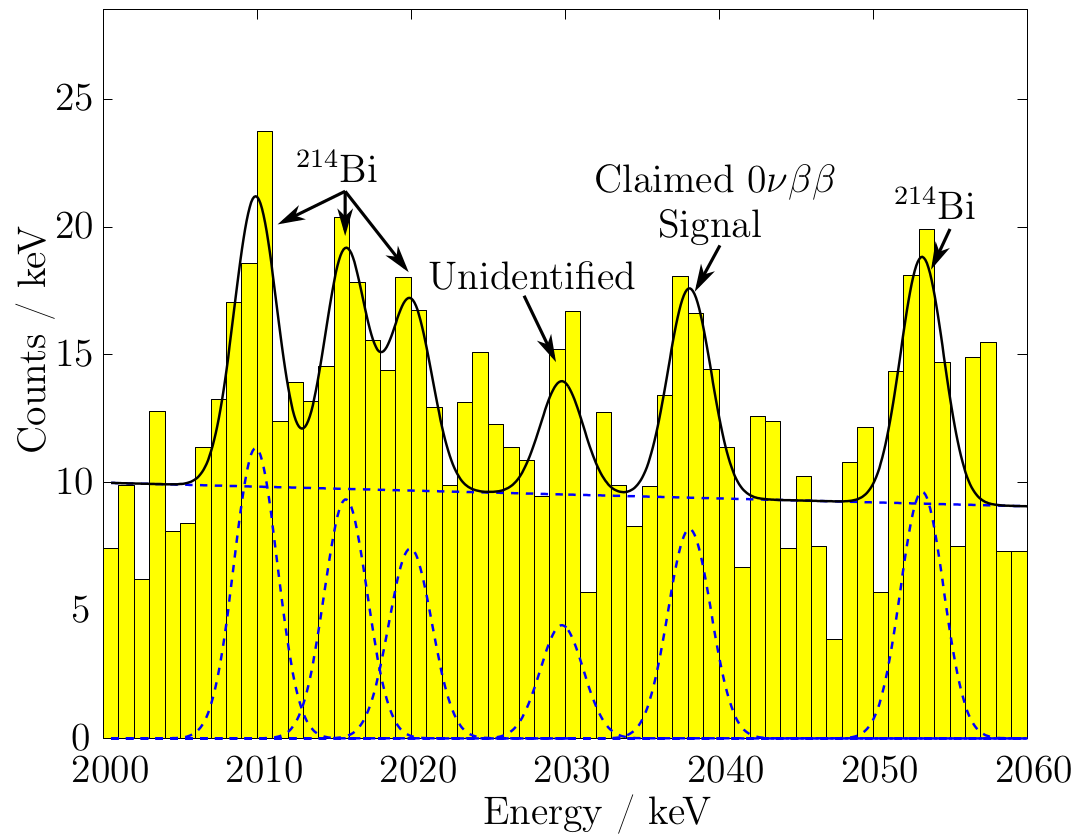
\includegraphics[scale=0.24]{pictures/Chap2/H-M-experiment-claim.png}
\caption{Total energy spectrum from the H-M experiment~\cite{HeidelbergMoscow1}. The peak at 2039~keV was claimed as a discovery of 0$\nu\beta\beta$ decay.}
\label{HMexperimentClaim}
\end{center}
\end{figure}


\FloatBarrier

\subsubsection{IGEX}


\NI The International GEmanium eXperiment (IGEX) was a similar experiment to H-M using 2.0~kg of $^{\text{76}}$Ge enriched to 86~\% distributed in six detectors. With an exposure of 8.9~kg~y of data, a limit on the half-life has been set to T$_{\text{1/2}}^{0\nu}$~>~1.57~$\times$~10$^{\text{25}}$~y which corresponds to $\langle \text{m}_{\beta\beta} \rangle$~<~280~-~550~meV~\cite{IGEX}.


\subsubsection{GERDA}


\NI The GERmanium Detector Array experiment (GERDA) uses a serie of HPGe detectors including 8 from the H-M and IGEX experiments with the intention of testing the claim of 0$\nu\beta\beta$ decay observation. 17.7~kg, along with 3.6~kg of new Broad Energy~Ge (BEGe) detectors was immersed in a 64~m$^\text{3}$ cryostat filled with liquid argon acting as a coolant and as a shielding. 3~m of water Cerenkov is added around to veto cosmic muons~\cite{GERDA}.


\bigskip 


\NI Installed at LNGS, GERDA took data, in a first phase, from November 2011 to May 2013 for a total exposure of 21.6~kg~y. No 0$\nu\beta\beta$ signal has been observed, and a limit of T$_{\text{1/2}}^{0\nu}$~>~2.1~$\times$~10$^{\text{25}}$~y has been set which corresponds to $\langle \text{m}_{\beta\beta} \rangle$~<~240~-~480~meV~\cite{GERDA}. In a second phase, 20~kg of enriched $^{\text{76}}$Ge have be added. GERDA collects data since December 2015 and no hint of 0$\nu\beta\beta$ signal has been found in the combined data as shown in Figure~\ref{GERDAresults}. A limit has been set to T$_{\text{1/2}}^{0\nu}$~>~5.3~$\times$~10$^{\text{25}}$~y at 90\% C.L. corresponding to $\langle \text{m}_{\beta\beta} \rangle$~<~150~-~330~meV.


\begin{figure}[h!]
\begin{center}
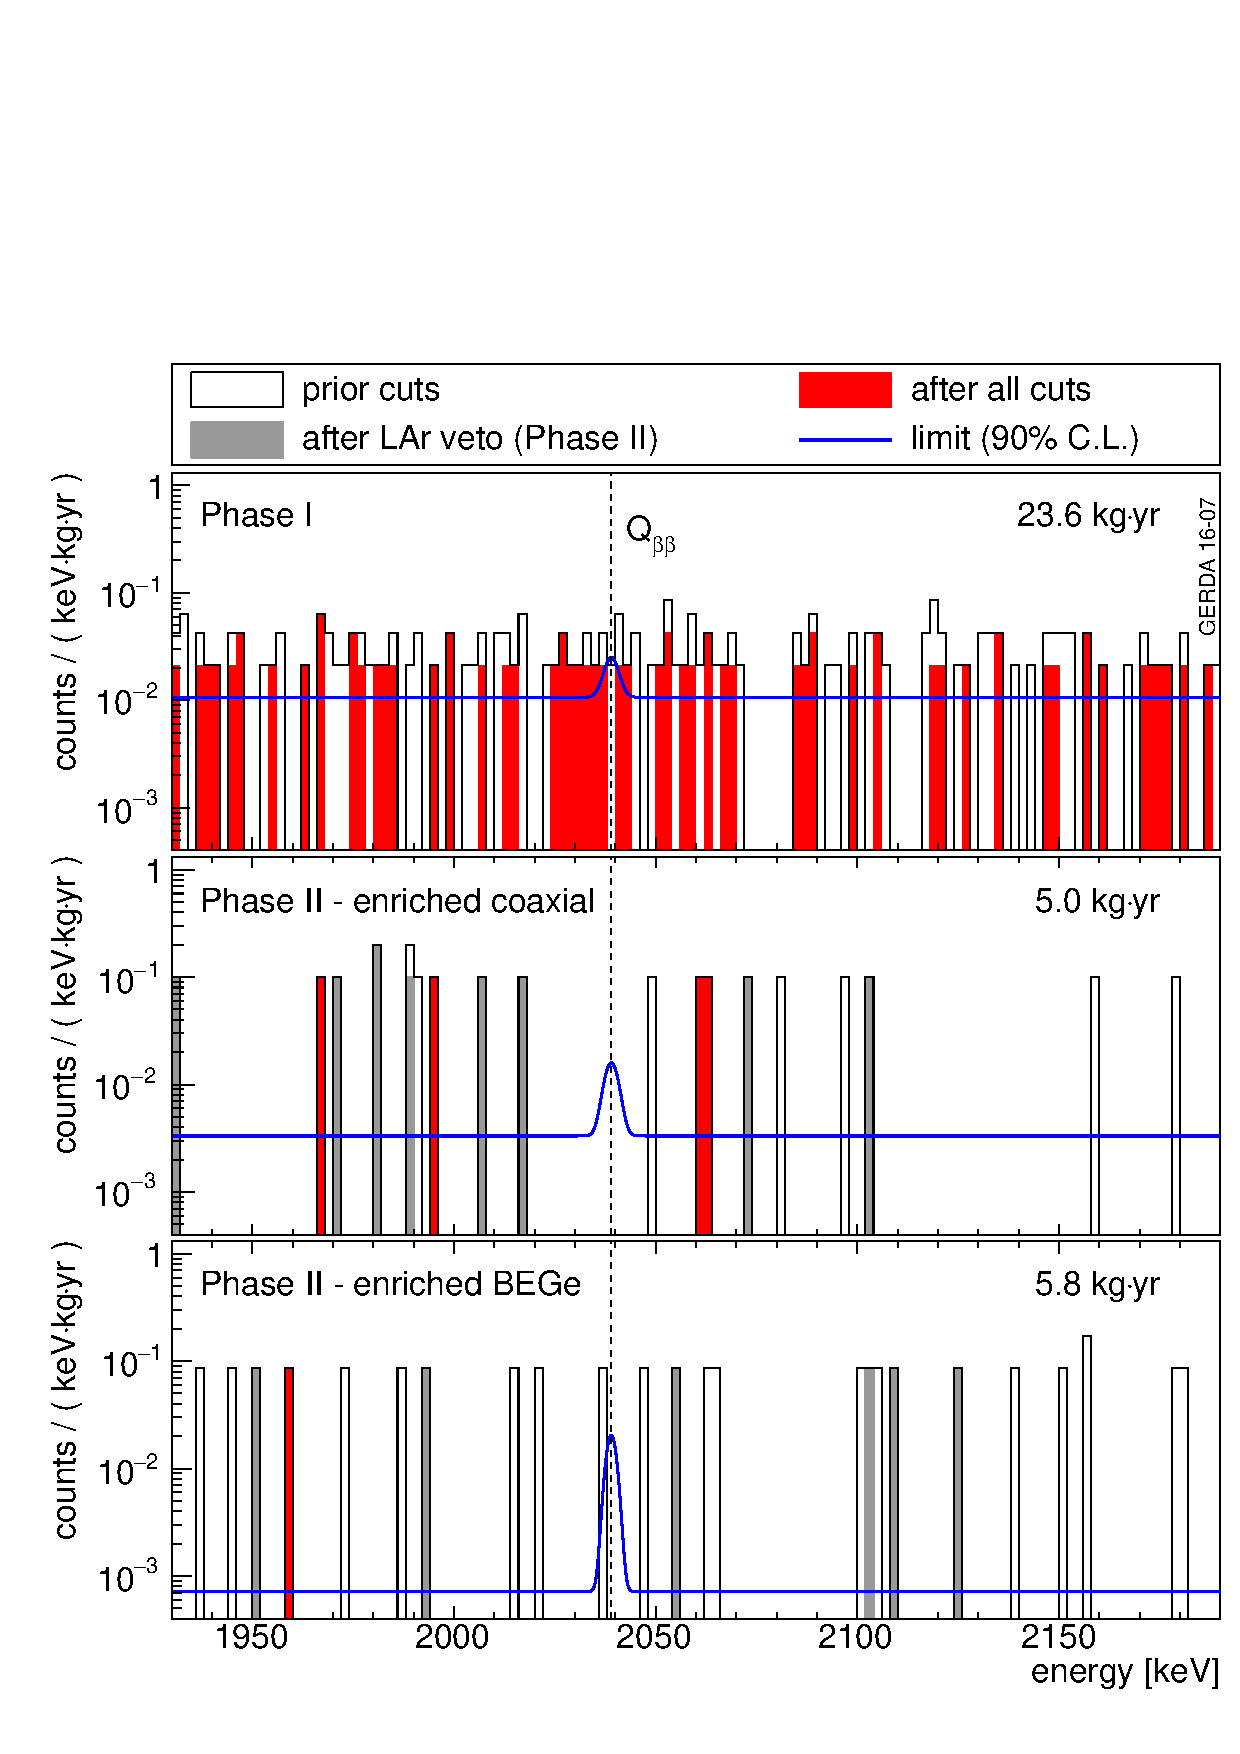
\includegraphics[scale=0.45]{pictures/Chap2/GerdaPhase2.pdf}
\caption{Combined Phase I data (top), Phase II coaxial (middle) and BEGe detector spectra (bottom) in the analysis window. The red histogram is the final spectrum, the filled grey one without pulse shape discrimination and the open one in addition without argon veto cut. The blue line is the fitted spectrum together with a hypothetical signal corresponding to the 90\% C.L. limit of T$_{\text{1/2}}^{0\nu}$~>~5.3~$\times$~10$^{\text{25}}$~y~\cite{GERDAphase2}.}
\label{GERDAresults}
\end{center}
\end{figure}


\FloatBarrier


\subsubsection{MAJORANA}


The MAJORANA experiment will also search for 0$\nu\beta\beta$ decays with enriched $^{\text{76}}$Ge crystals. This experiment expects to surpass the sensitivity of H-M and IGEX by improving the radiopurity of the detector materials, by using more effective shieldings and by increasing the background-signal discrimination. Their aims are to achieve an energy resolution better than 3~keV and a very low background rate of 1~count/tonne/y in the ROI. A demonstrator module (MJD) is currently operating at the Sanford Underground Research Facility to show that the background levels can be achieved and extended to a tonne-scale experiment. If the desired background levels are achieved with the demonstrator, a sensitivity of $\langle \text{m}_{\beta\beta} \rangle$~<~80~-~160~meV can be reached after 2.5~y of data taking~\cite{MAJORANA}.


\bigskip


\NI The GERDA and MAJORANA collaborations are strongly connected. Depending on their results, there is a possibility of merging the two projects to build an experiment containing 1~tonne of $^{\text{76}}$Ge to reach a sensitivity of $\langle \text{m}_{\beta\beta} \rangle$~<$\sim$~10~meV~\cite{MAJORANAandGERDA} \\

\subsubsection{COBRA}


\NI Most of the semiconductor experiments use germanium detectors but other semiconductor technologies can provide competitive results. The COBRA experiment (Cadmium Zinc Telluride 0-neutrino double-Beta Research Apparatus) runs at LNGS and searches for 0$\nu\beta\beta$ decays among 5 $\beta\beta$ isotopes ($^{\text{70}}$Zn,$^{\text{114}}$Cd,$^{\text{116}}$Cd,$^{\text{128}}$Te and $^{\text{130}}$Te) with an array of CdZnTe semiconductors. The energy resolution of this semiconductor is not as good as with HPGe experiments ($\sim$ 30~keV at 2800~keV) but it operates at room temperature. Thanks to the pixellated array, the tracking and identification of the particles are possible which reduces the background level ($\sim$ 1~count/keV/kg/y at 2800~keV is expected). In its demonstrator phase, COBRA comprises 64 CdZnTe coplanar-grid semiconductor detectors arranged in 4$\times$4 detectors. After an exposure of 234.7~kg.d no signal of 0$\nu\beta\beta$ has been found. The limits set on the five isotopes are reported in Table~\ref{tab:CobraResultsDemonstrator} such as their Q$_{\beta\beta}$ value and the measured background for the different R.O.I.~\cite{CobraDemonstrator}.


\begin{table}[h!]
\centering
\begin{tabular}{c|c|c|c}
\toprule
Isotope & Q$_{\beta\beta}$ [keV] & b [cts./keV/kg/yr] & T$_{\text{1/2}}^{0\nu}$ [$\times$ 10$^{\text{21}}$~y] at 90\% C.L. \\[0.1cm]
\hline
$^{\text{70}}$Zn  & 997  & 4.51$^{+\text{0.6}}_{-\text{1.0}}$  & 6.8 $\times$ 10$^{-\text{3}}$ \\[0.1cm]
$^{\text{114}}$Cd & 543  & 219.9$^{+\text{1.0}}_{-\text{1.7}}$ & 1.6 \\[0.1cm]
$^{\text{116}}$Cd & 2814 & 2.7$^{+\text{0.1}}_{-\text{0.2}}$   & 1.1 \\[0.1cm]
$^{\text{128}}$Te & 867  & 65.5$^{+\text{0.5}}_{-\text{1.6}}$  & 1.9 \\[0.1cm]
$^{\text{130}}$Te & 2528 & 3.6$^{+\text{0.1}}_{-\text{0.3}}$   & 6.1 \\[0.1cm]
\bottomrule
\end{tabular}
\caption{Results on the 0$\nu\beta\beta$ half-life decay rate of the COBRA in its demonstrator phase.}
\label{tab:CobraResultsDemonstrator}
\end{table}

%The experiment is in a R\&D phase to increase the energy resolution and reduce the background rate in order to reach a sensitivity of $\langle \text{m}_{\beta\beta} \rangle$~<~50~-~70~meV with 420~kg~\cite{COBRA}.


\subsection{Scintillation experiments}


\NI Scintillation experiment consists of scintillating materials doped with $\beta\beta$ isotopes. It can be either in an organic crystal form or in large volume of liquid scintillator. The particles emitted during a decay excite the scintillating medium which re-emits the absorbed energy as scintillation light. This light is then usually detected by an array of PMTs. This kind of detector have the advantages to be relatively inexpensive and have a high degree of radiopurity. 


\bigskip


%\NI Two sorts of scintillation experiments exist. In the first one, the $\beta\beta$ isotope is inherently a part of the scintillator as was the case in the ELEGANT~V experiment. In the second one, a large volume of liquid scintillator is used in which a $\beta\beta$ isotope is dissolved. This second type suffers from poor energy resolution but the mass of isotopes can be readily increased to study a large scale volume.



\subsubsection{ELEGANT VI}


\NI Operating in Kamioka, the ELEGANT VI experiment searched for 0$\nu\beta\beta$ decay in 23 CaF$_\text{2}$(Eu) crystal scintillators with 7.6~g of enriched~$^{\text{48}}$Ca. With an exposure of 0.015~kg~y, the experiment sets a limit on the half-life to be T$_{\text{1/2}}^{0\nu}$~>~5.8~$\times$~10$^{\text{22}}$~y corresponding to~$\langle \text{m}_{\beta\beta} \rangle$~<~3.2~-~22~meV~\cite{ELEGANTVI}.


\subsubsection{CANDLESIII}


\NI The CANDLES experiment operates in Kamioka and consists of 305~CaF$_\text{2}$ crystals, for a total mass of 305~kg, placed in a liquid scintillator surrounded by PMTs. The experiment is currently taking data and a sensitivity of $\langle \text{m}_{\beta\beta} \rangle$~$\sim$~500~eV is expected~\cite{CANDLESIII}.


\subsubsection{Aurora}


\NI The Aurora experiment investigates the double beta decay of $^{\text{116}}$Cd using 1.162~kg of Cadmium Tungstate crystal scintillators enriched in $^{\text{116}}$Cd to 82\%. The experiment is installed in the low DAMA/R\&D setup operated at the LNGS in Italy. In its last configuration, the CdW0$_\text{4}$ crystal scintillators are fixed in polytetrafluoroethylene containers filled with ultrapure liquid scintillator in order to improve the light collection and acting as an anti-coincidence veto counter. The energy resolution of the detector is 5\% (FWHM) at 2.6~MeV. The Aurora experiment measured the 2$\nu\beta\beta$ half-life of~$^{\text{116}}$Cd to be 2.62~$\pm$~0.14~$\times$~10$^{\text{19}}$~y with a signal to background ratio of 2.6/1 in the energy interval (1.1 - 2.8) MeV. The Aurora experiment also performs the search for the 0$\nu\beta\beta$. No signal has been found and limit of the half life has been set to 1.9 $\times$ 10$^{\text{23}}$~y corresponding to~$\langle \text{m}_{\beta\beta} \rangle$~<~(1.2~-~1.8)~eV~\cite{AuroraRecent}.  


\subsubsection{KamLAND-Zen}


\NI KamLAND-Zen is an experiment that uses the KamLAND detector which was built to study the neutrino oscillation. The experiment searches for the 0$\nu\beta\beta$ decay in~$^{\text{136}}$Xe, with 13 tonnes of liquid scintillator doped with $^{\text{136}}$Xe suspended in a nylon balloon at the center of the KamLAND detector. This inner balloon is surrounded by an outer balloon containing 1000~tonnes of liquid scintillator which is used as an active shield against external sources of $\gamma$-rays. Around the two balloons a stainless steel tank is instrumented with $\sim$~2000~PMTs to detect the scintillation light.


\bigskip


\NI In a first phase the experiment identified an unexpected background contributions in the 0$\nu\beta\beta$~ROI coming from the surface of the inner balloon. These backgrounds are attributed to the radioactive fallout from the Fukushima accident. The experiment decided to halt in order to purify the inner balloon. The experiment restarted after the balloon purification for a second phase, and reaches by combining the two phases a limit for the 0$\nu\beta\beta$ decay half-life of T$_{\text{1/2}}^{0\nu}$~>~1.06~$\times$~10$^{\text{26}}$~y corresponding to~$\langle \text{m}_{\beta\beta} \rangle$~<~61~-~165~meV which is the strongest single constraint on $\langle \text{m}_{\beta\beta} \rangle$ for any isotope~\cite{KamLAND-ZenRecent}.    


%Despite this unexpected contamination, KamLAND-Zen still provides the strongest single constraint on $\langle \text{m}_{\beta\beta} \rangle$ for any isotope. With an exposure of 89.5~kg~y, a limit of T$_{\text{1/2}}^{0\nu}$~>~1.9~$\times$~10$^{\text{25}}$~y corresponding to~$\langle \text{m}_{\beta\beta} \rangle$~<~120~-~250~meV is obtained~\cite{KamLAND-Zen}.


%KamLAND-Zen2 Majoron emission \cite{KamLAND-Zen2} \\

\begin{figure}[h!]
\begin{center}
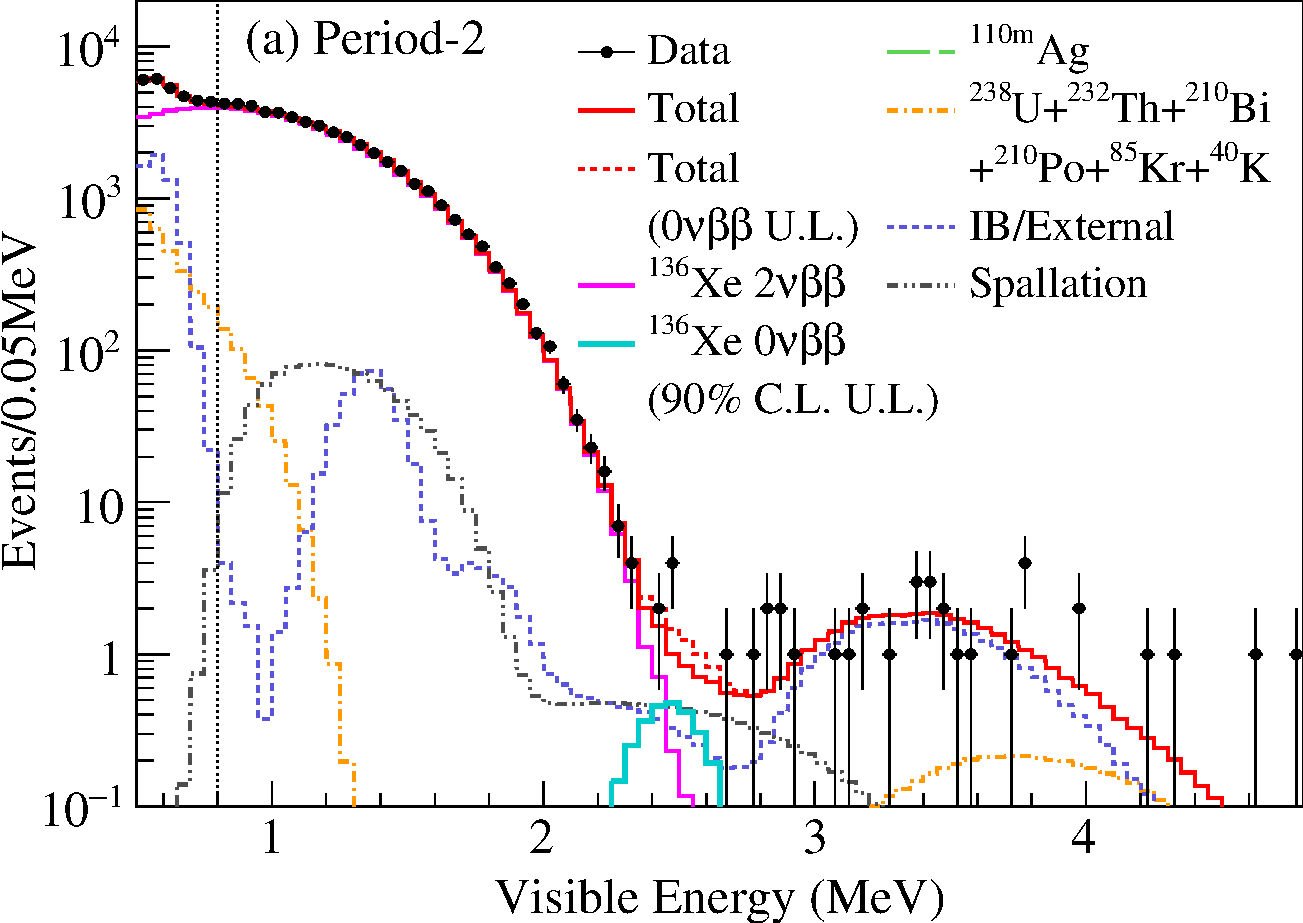
\includegraphics[scale=0.5]{pictures/Chap2/fig2a.pdf}
%\caption{Energy spectrum showing the first result from KamLAND-Zen. The considerable background at 2.46~MeV was not expected to be so high, in particular $^{\text{111m}}$Ag~\cite{KamLAND-Zen}.}
\caption{Energy spectrum of the selected $\beta\beta$ candidates.}
\label{KamLANDZenResults}
\end{center}
\end{figure}



\NI In a future phase of the experiment, the detector will be upgraded to contain 1~tonne of $^{\text{136}}$Xe with an improvement of the light collection. The expected sensitivity is $\langle \text{m}_{\beta\beta} \rangle$~$\sim$~20~meV~\cite{KamLAND-Zen3}.


\FloatBarrier


\subsubsection{SNO+}


\NI The SNO+ experiment follows the same principle as KamLAND-Zen. The experiment will operate in SNOlab and will reuse the acrylic sphere used in the SNO experiment. In a first phase, 800~kg of~$^{\text{130}}$Te, will be dissolved in 780~tonnes of liquid scintillator and introduced in the 12~m diameter sphere. Approximately 9500 PMTs will be used to read out the scintillation light. With 5~y of data taking, SNO+ will reach a sensitivity of $\langle \text{m}_{\beta\beta} \rangle$~<~55~-~133~meV. In a second phase, the mass of $^{\text{130}}$Te could be increased by a factor 10 and provide sensitivity up to  $\langle \text{m}_{\beta\beta} \rangle$~<~19~-~46~meV~\cite{SNO+}.


\subsection{Bolometer experiments}


\NI The bolometer experiments detect the ionizing radiations by measuring small increases in temperature of a material. The increase of the temperature changes the electrical properties of the medium which can be measured and related to the ionizing particle energy. These detectors operate at very low temperature, of the order of~mK, to obtain very good energy resolution. They measure only the total energy deposited by the particle and does not have good particle identification capabilities makink difficult the background identification.


\subsubsection{CUORE}


\NI The CUORICINO experiment was a prototype of the CUORE experiment (Cryogenic Underground Observatory for Rare Events). It ran at LNGS between 2003 and 2008, and searched for 0$\nu\beta\beta$ decay in 507~g of~$^{\text{130}}$Te.  The experiment consisted of a tower array of 62~Te0$_\text{2}$ crystals placed in a cryostat. With a total of 19.75~kg~y, a limit has been set to T$_{\text{1/2}}^{0\nu}$~>~2.8~$\times$~10$^{\text{24}}$~y corresponding to $\langle \text{m}_{\beta\beta} \rangle$~<~300~-~700~meV~\cite{CUORICINO}.


\bigskip


\NI CUORE is the next generation experiment extending the CUORICINO concept to a larger array of bolometers. The full CUORE detector contains 988 Te0$_\text{2}$ crystals (204~kg of~$^{\text{130}}$Te) to reach an expected sensitivity of T$_{\text{1/2}}^{0\nu}$~>~2.1~$\times$~10$^{\text{26}}$~y corresponding to $\langle \text{m}_{\beta\beta} \rangle$~<~35~-~82~meV. A demonstrator module, CUORE-0, consisting of 52 crystals and 10.7~kg of $^{\text{130}}$Te is currently running. A first limit has been set to T$_{\text{1/2}}^{0\nu}$~>~8~$\times$~10$^{\text{24}}$~y which corresponds to $\langle \text{m}_{\beta\beta} \rangle$~<~270~-~760~meV~\cite{CUORE}.


\subsection{Scintillating bolometer experiments}


New detectors will implement scintillating bolometers that simultaneously detect temperature changes and scintillation light. The combination of these two observables can be used for particle identification and to allow a better background rejection.  


\subsubsection{LUCIFER}


\NI LUCIFER (Low background Underground Cryogenics Installation for Elusive Rates) is an experiment which uses ZnSe crystals that act as both a bolometer and a scintillator. The combination of temperature and scintillation light measurements can be used for particle identification and allow a better background rejection. The crystals will contain $\sim$~18~kg of $^{\text{82}}$Se to reach a sensitivity of $\langle \text{m}_{\beta\beta} \rangle$~$\sim$~60~meV~\cite{LUCIFER} after years of data taking. This detector will serve as a prototype for the CUPID experiment (Cuore Upgrade with Particle IDentification) which is in the early phases of R\&D.


\subsubsection{LUMINEU}


\NI The Luminescent Underground Molybdenum Investigation for NEUtrino mass and nature (LUMINEU) is a French R\&D program to search for 0$\nu\beta\beta$ decay of $^{\text{100}}$Mo by using scintillating bolometer technique~\cite{LUMINEU}. The LUMINEU project aims to develop high-quality radiopure ZnMoO$_\text{4}$ crystals crystal scintillators of large mass (300 - 500~g) and test them as low-temperature detectors. The main aim of the project is to demonstrate feasibility of ZnMoO$_\text{4}$ based  cryogenic scintillating  bolometers for the future 0$\nu\beta\beta$ generation experiment. The LUMINEU project could lead to an experiment containing approximately 10~kg of $^{\text{100}}$Mo. A sensitivity of such experiment could reach a sensitivity on the 0$\nu\beta\beta$ half-life on the level of the best current experiments. By scaling up to the 100-1000~kg experiment could entirely cover the inverted ordering region~\cite{LUMINEU}.



\subsection{Time projection chamber experiments}


\NI The time projection chamber (TPC) experiments are a type of detector using gaseous or liquid medium combined with an electric field. By crossing the detector, charged particles ionize the medium and produce free electrons. These free electrons are drifted towards segmented collection planes called anodes. The generated current at the anode is proportional to the energy of the initial radiation. Since the anode is segmented, the position can be reconstructed in two-dimensions. The measurement of the arrival times on the anode plane provide information which can be translated into a third position coordinate. As a result, TPC detectors can reconstruct the particle track in three-dimensions which is used to search for common vertex from two electrons.


\bigskip


\NI The most common isotope for $\beta\beta$ decay studies with TPC is $^{\text{136}}$Xe, which also has the advantage of providing both ionization and scintillation signals. This scintillation light can be used to perform more accurate energy measurement than what is possible with the ionization signal alone.    


\subsubsection{EXO}


\NI The Enriched Xenon Observatory (EXO) experiment is a liquid xenon TPC looking for 0$\nu\beta\beta$ decay in~$^{\text{136}}$Xe. The experiment is housed in the Waste Isolation Pilot Plant (WIPP) located at New Mexico, USA. The first prototype, EXO-200, is a cylindrical homogeneous TPC filled with liquid xenon, including 80~kg of~$^{\text{136}}$Xe, which is currently running. The detector uses the scintillation and ionization signals to reconstruct event topologies. It is symmetric around a central cathode plane. The two end caps are instrumented with wire anode grids and avalanche photodiodes to respectively read out the ionization and scintillation signals. The TPC is surrounded by a cryostat, a lead shielding and a plastic scintillator array to reject cosmic rays. After having recorded an exposure of 100~kg~y, no signal of 0$\nu\beta\beta$ decay has been found. A limit of T$_{\text{1/2}}^{0\nu}$~>~1.1~$\times$~10$^{\text{25}}$~y, corresponding to $\langle \text{m}_{\beta\beta} \rangle$~<~190~-~450~meV~have been set~\cite{EXO-200}. 


\bigskip


\NI In the future, the EXO experiment could be scaled up to the tonne scale. A new technique to tag the $^{\text{136}}$Ba ions, daughter of the $^{\text{136}}$Xe, is investigated to reduce the background level. With a tonne scale experiment, a sensitivity of T$_{\text{1/2}}^{0\nu}$~>~2~$\times$~10$^{\text{27}}$~y, corresponding to $\langle \text{m}_{\beta\beta} \rangle$~<~15~-~32~meV could be achieved.


%\begin{figure}[h!]
%\begin{center}
%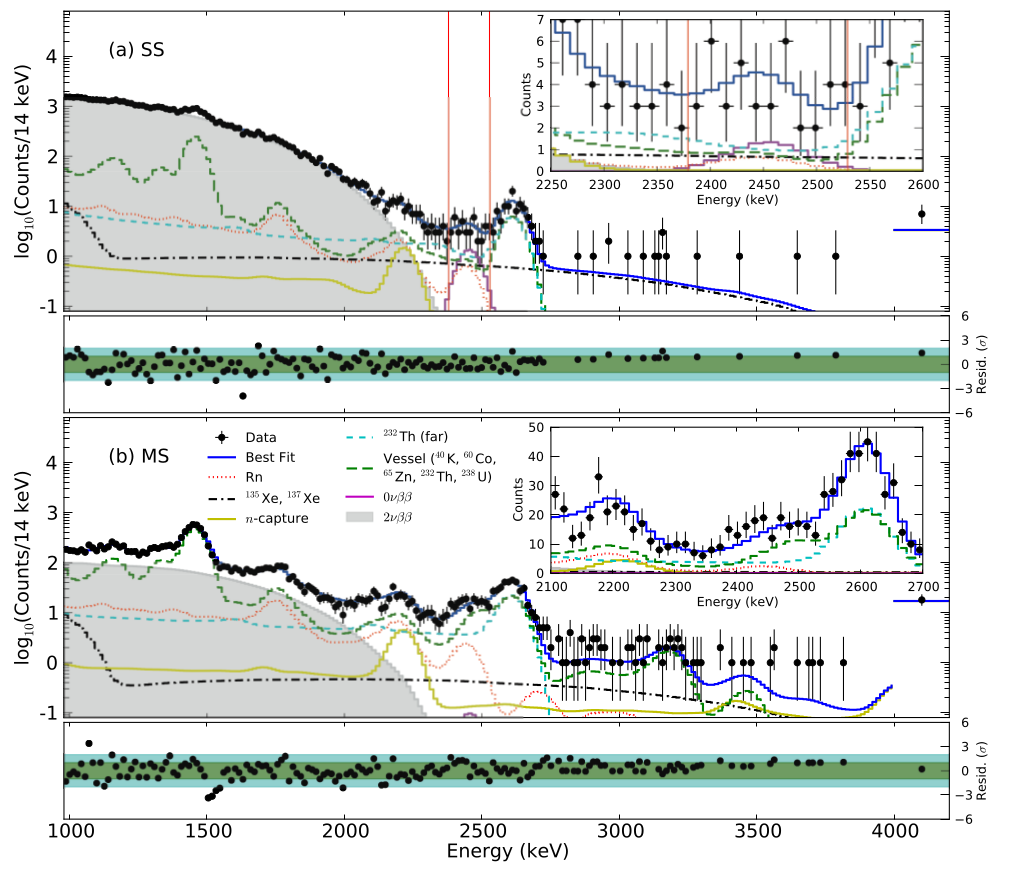
\includegraphics[scale=0.4]{pictures/Chap2/EXO-200-experiment.png}
%\caption{Energy spectrum showing the results from EXO-200. Events in the detector are classifed as single-site (SS) or multi-site (MS) according to the number of detected charge deposits. 0$\nu\beta\beta$ events are predominantly SS whereas backgrounds are mostly MS. The results for the SS event are shown in the top while the MS event are shown in the bottom plot. No signal of 0$\nu\beta\beta$ decay appear.}
%\label{EXO200results}
%\end{center}
%\end{figure}


\FloatBarrier


\subsubsection{NEXT}


\NI The Neutrino Experiment with a Xenon TPC experiment (NEXT) is an experiment which is under construction in the Canfranc Underground Laboratory in Spain, looking for 0$\nu\beta\beta$ decays in~$^{\text{136}}$Xe. It consists of a cylindrical TPC using gaseous xenon at high pressure. The detector will detect both scintillation and ionization signals. The scintillation light will be detected by PMTs at one end cap while the ionization signal will be amplified and produce electroluminescence that can be read out by silicon PM. This second signal provides tracking information and allows improvement of the energy resolution. A prototype detector, NEXT-100, with 100~kg of~$^{\text{136}}$Xe is currently operating, a sensitivity of T$_{\text{1/2}}^{0\nu}$~>~1.9~$\times$~10$^{\text{25}}$~y is expected corresponding to $\langle \text{m}_{\beta\beta} \rangle$~<~70~-~150~meV~\cite{NEXT}. The advantage of NEXT-100 is that it is readily scalable. If the prototype is succesfull, it is possible to enlarge it to contain a tonne of material to reach a sensitivity of $\langle \text{m}_{\beta\beta} \rangle$~<~15~-~32~meV.



\subsection{Tracker-calorimeter experiments}


\NI The tracker-calorimeter experiments separate the $\beta\beta$ isotope from the detection device which allows to investigate the $\beta\beta$ decay for many candidate isotope. The track of the two electrons and their energy are measured by two disctinct detectors. This technique allows to reconstruct the full topology and kinematics of individual particles within an event, which results in excellent background rejection and also gives the possibility to distinguish the mechanism behind the 0$\nu\beta\beta$ decay. However, the tracker-calorimeter experiments, due to the separation of the isotope from the rest of the detector, generally suffer from lower energy resolution and detection efficiency compared to the other type of $\beta\beta$ detectors. The most renowned experiments using tracker-calorimeter technique are the NEMO-3 experiment and its successor SuperNEMO. They will be described in more details in Chapter~\ref{chap:NEMO}.


\section{Summary and status of the $\beta\beta$ researches}\label{sec:StatusDBD}


\NI Today, the direct measurement of the 2$\nu\beta\beta$ decay has been made for nine isotopes. The most accurate measurements to date are presented in Table~\ref{tab:summaryBB2NUmeasurements}. Due to its ability to measure different isotopes, NEMO-3 is often quoted. $^{\text{76}}$Ge and $^{\text{136}}$Xe have been measured by GERDA-I and EXO-200 respectively.


\bigskip


\NI No evidence of 0$\nu\beta\beta$ decay has been observed whatever the isotope. The best half-life limits are given in Table~\ref{tab:summaryBB0NUmeasurements}. The best limit on $\langle \text{m}_{\beta\beta} \rangle$ has been set by the KamLAND-Zen experiment.


\bigskip


\NI When different experiments investigate the same isotope, their results can be combined to obtain a stronger half-life limit. For example, by combining the GERDA results with H-M and IGEX, a limit of T$_{\text{1/2}}^{\text{0}\nu}$ > 3.0 $\times$ 10$^{\text{25}}$~y corresponding to $\langle \text{m}_{\beta\beta} \rangle$ < 0.20 - 0.40~eV can be set~\cite{GERDA}.  By combining the results on $^{\text{136}}$Xe from EXO-200 and KamLAND-Zen, the sensitivity is set to T$_{\text{1/2}}^{\text{0}\nu}$ > 3.4 $\times$ 10$^{\text{25}}$~y which corresponds to $\langle \text{m}_{\beta\beta} \rangle$ < 0.12 - 0.25~eV~\cite{KamLAND-Zen}. These results can be summarised in a plot showing the sensitivity on $^{\text{76}}$Ge versus the sensitivity of $^{\text{136}}$Xe for different NME calculations as shown in Figure~\ref{Gerda-EXO-combined}. Both results strongly disfavor the H-M claim. The results obtained on the effective neutrino mass for the different isopotes are represented in Figure~\ref{KamLAND-Zen-results}. To date the best limit on the effective neutrino mass has been obtained with the $^{\text{136}}$Xe by KamLAND-Zen experiment.


\bigskip


\NI Today, several new experiments are planned to search for 0$\nu\beta\beta$ process as listed in Table~\ref{tab:futureBBexperiment}. Some of them are currently running while others are finishing their R\&D phase or are in construction stage. These new experiments are expected to approach the parameter space for the inverted hierarchy. Many of them plan to scale up to larger mass to fully explore the inverted hierarchy parameter space at $ \langle \text{m}_{\beta\beta} \rangle$~$\sim$10~meV. In a scenario in which nature has chosen the inverted hierarchy for neutrino masses, these experiments will either discover or exclude the 0$\nu\beta\beta$ decay.


\begin{table}[h!]
\centering
\begin{tabular}{cccc}
\toprule
Isotope & Experiment & T$_{\text{1/2}}^{\text{2}\nu}$~[$\times$ 10$^{\text{19}}$y]& Ref. \\
\midrule
$^{\text{48}}$Ca  & NEMO-3  & 6.4$^{+\text{0.6}}_{-\text{0.7}}$ $^{+\text{1.2}}_{-\text{0.9}}$ & \cite{NEMO3:Ca48} \\[0.1cm]
$^{\text{76}}$Ge  & GERDA-I & 192.6$^{+\text{2.5}}_{-\text{2.2}}$ $\pm$ 9.2 & \cite{Gerda2nubb} \\[0.1cm]
$^{\text{82}}$Se  & NEMO-3  & 9.93 $\pm$ 0.14 $\pm$ 0.72 & \cite{ThesisJMott} \\[0.1cm]
$^{\text{96}}$Zr  & NEMO-3  & 2.35 $\pm$ 0.14 $\pm$ 0.16 & \cite{NEMO3:Zr96} \\[0.1cm]
$^{\text{100}}$Mo & NEMO-3  & 0.711 $\pm$ 0.002 $\pm$ 0.054 & \cite{NEMO3:Mo100-pre} \\[0.1cm]
%$^{\text{116}}$Cd & NEMO-3  & 2.74 $\pm$ 0.04 $\pm$ 0.18 & \cite{Arnold2016bed} \\[0.1cm]
$^{\text{116}}$Cd & Aurora  & 2.62 $\pm$ 0.14     & \cite{AuroraRecent} \\[0.1cm]
$^{\text{130}}$Te & NEMO-3  & 70 $\pm$ 9 $\pm$ 11 & \cite{NEMO3:Te130} \\[0.1cm]
$^{\text{136}}$Xe & EXO-200 & 216.5 $\pm$ 1.6 $\pm$ 5.9 & \cite{EXO-200-2nubb} \\[0.1cm]
$^{\text{150}}$Nd & NEMO-3  & 0.934 $\pm$ 0.022$^{+\text{0.060}}_{-\text{0.059}}$  & \cite{NEMO3:Nd150} \\
\bottomrule
\end{tabular}
\caption{Most accurate measurements of the 2$\nu\beta\beta$ half-life. The first error corresponds to the statistical and the second is systemtic}
\label{tab:summaryBB2NUmeasurements}
\end{table}



\begin{table}[h!]
\centering
\begin{tabular}{cccccc}
\toprule
Isotope & Experiment & Exposure [kg.y]& T$_{\text{1/2}}^{\text{0}\nu}$~[y] & $\langle \text{m}_{\beta\beta} \rangle$ [eV]&  Ref. \\
\midrule
$^{\text{48}}$Ca  & ELEGANT VI       & 0.015 & 5.8 $\times$ 10$^{\text{22}}$ & 3.5 - 22    & \cite{ELEGANTVI}       \\[0.1cm]
$^{\text{76}}$Ge  & GERDA-I          & 16.4  & 2.1 $\times$ 10$^{\text{25}}$ & 0.24 - 0.48 & \cite{GERDA}           \\[0.1cm]
$^{\text{82}}$Se  & NEMO-3           & 4.90  & 2.2 $\times$ 10$^{\text{23}}$ & 1.0 - 2.8   & \cite{ThesisJMott}     \\[0.1cm]
$^{\text{96}}$Zr  & NEMO-3           & 0.031 & 9.2 $\times$ 10$^{\text{21}}$ & 7.2 - 19.5  & \cite{NEMO3:Zr96}      \\[0.1cm]
$^{\text{100}}$Mo & NEMO-3           & 34.5  & 1.1 $\times$ 10$^{\text{24}}$ & 0.33 - 0.62 & \cite{NEMO3:Mo100}     \\[0.1cm]
$^{\text{116}}$Cd & Aurora           & 1.31  & 1.9 $\times$ 10$^{\text{23}}$ & 1.2 - 1.8   & \cite{AuroraRecent}    \\[0.1cm]
$^{\text{130}}$Te & CUORICINO/CUORE  & 19.75 & 4.0 $\times$ 10$^{\text{24}}$ & 0.27 - 0.76 & \cite{CUORE-TeResults} \\[0.1cm]
$^{\text{136}}$Xe & KamLAND-Zen      & 89.5  & 1.9 $\times$ 10$^{\text{25}}$ & 0.12 - 0.25 & \cite{KamLAND-Zen}     \\[0.1cm]
$^{\text{150}}$Nd & NEMO-3           & 0.19  & 2.0 $\times$ 10$^{\text{22}}$ & 1.6 - 5.3   & \cite{NEMO3:Nd150}     \\
\bottomrule
\end{tabular}
\caption{Best half-life limits obtained from individual experiments from different 0$\nu\beta\beta$ isotopes. All the limits are given at 90\% CL.}
\label{tab:summaryBB0NUmeasurements}
\end{table}

% expoure Aurora : (1.162*0.82)kg * (12015)hours


\begin{figure}[h!]
\begin{center}
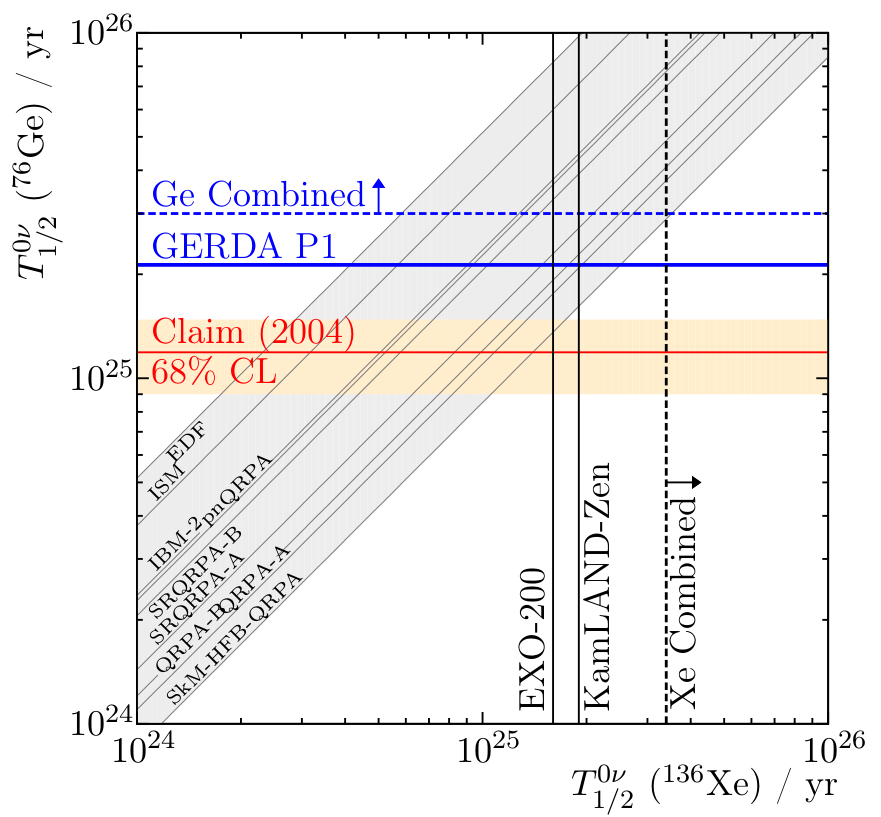
\includegraphics[scale=0.30]{pictures/Chap2/Gerda-EXO-combined.png}
\caption{Limits on T$_{\text{1/2}}^{\text{2}\nu}$ for $^{\text{76}}$Ge from GERDA-I and $^{\text{136}}$Xe from EXO-200 and KamLAND-Zen compared with the claim of 0$\nu\beta\beta$ from H-M experiment.}
\label{Gerda-EXO-combined}
\end{center}
\end{figure}






\begin{table}
\centering
\begin{tabular}{lccccc}
\toprule
Experiment & Isotope & Mass [kg] & Type & $ \langle \text{m}_{\beta\beta} \rangle$~[meV] & Ref \\ 
\midrule
GERDA-II     & $^{\text{76}}$Ge  & 40   & Semiconductor & 50 - 100  & \cite{GERDA}        \\
MAJORANA     & $^{\text{76}}$Ge  & 40   & Semiconductor & 80 - 160  & \cite{MAJORANA}     \\
CANDLES III  & $^{\text{48}}$Ca  & 0.3  & Scintillator  & 500       & \cite{CANDLESIII}   \\
KamLAND-Zen  & $^{\text{136}}$Xe & 640  & Liquid Scint. & 40 - 85   & \cite{KamLAND-Zen3} \\
SNO+ (0.3\%) & $^{\text{130}}$Te & 800  & Liquid Scint. & 50 - 100  &  \\
CUORE-0      & $^{\text{130}}$Te & 10.7 & Bolometer     & 180 - 420 & \cite{CUORE}        \\
EXO-200      & $^{\text{136}}$Xe & 80   & Scint. TPC    & 85 - 180  & \cite{EXO-200}      \\
NEXT-100     & $^{\text{136}}$Xe & 90   & Scint. TPC    & 70 - 150  & \cite{NEXT}         \\
SuperNEMO    & $^{\text{82}}$Se  & 100  & Tracker-Calo  & 50 - 100  &  \\
\midrule
1ton Ge      & $^{\text{76}}$Ge  & 1000 & Semiconductor & 10        & - \\
COBRA        & $^{\text{116}}$Cd & 420  & Semiconductor & 50 - 70   & \cite{COBRA}        \\
CANDLES      & $^{\text{48}}$Ca  & 3    & Scintillator  & 50        & \cite{CANDLESIII}   \\
KamLAND2-Zen & $^{\text{136}}$Xe & 1000 & Liquid Scint. & 20        & \cite{KamLAND-Zen3} \\
SNO+ (3.0\%) & $^{\text{130}}$Te & 8000 & Liquid Scint. & 20 - 40   & - \\
CUORE        & $^{\text{130}}$Te & 204  & Bolometer     & 35 - 82   & \cite{CUORE}        \\
LUCIFER      & $^{\text{82}}$Se  & 18   & Scint. Bolom. & 60        & \cite{LUCIFER}      \\
EXO          & $^{\text{136}}$Xe & 1000 & Scint. TPC    & 15 - 62   & \cite{EXO-200}      \\
NEXT         & $^{\text{136}}$Xe & 1000 & Scint. TPC    & 15 - 62   & \cite{NEXT}         \\
\bottomrule
\end{tabular}
\caption{Summary of future $\beta\beta$ experiments. The top panel presents the experiments which are either running or under construction. The bottom panel shows experiments that have been proposed as successors to the current generation.}
\label{tab:futureBBexperiment}
\end{table}





\begin{figure}[h!]
\begin{center}
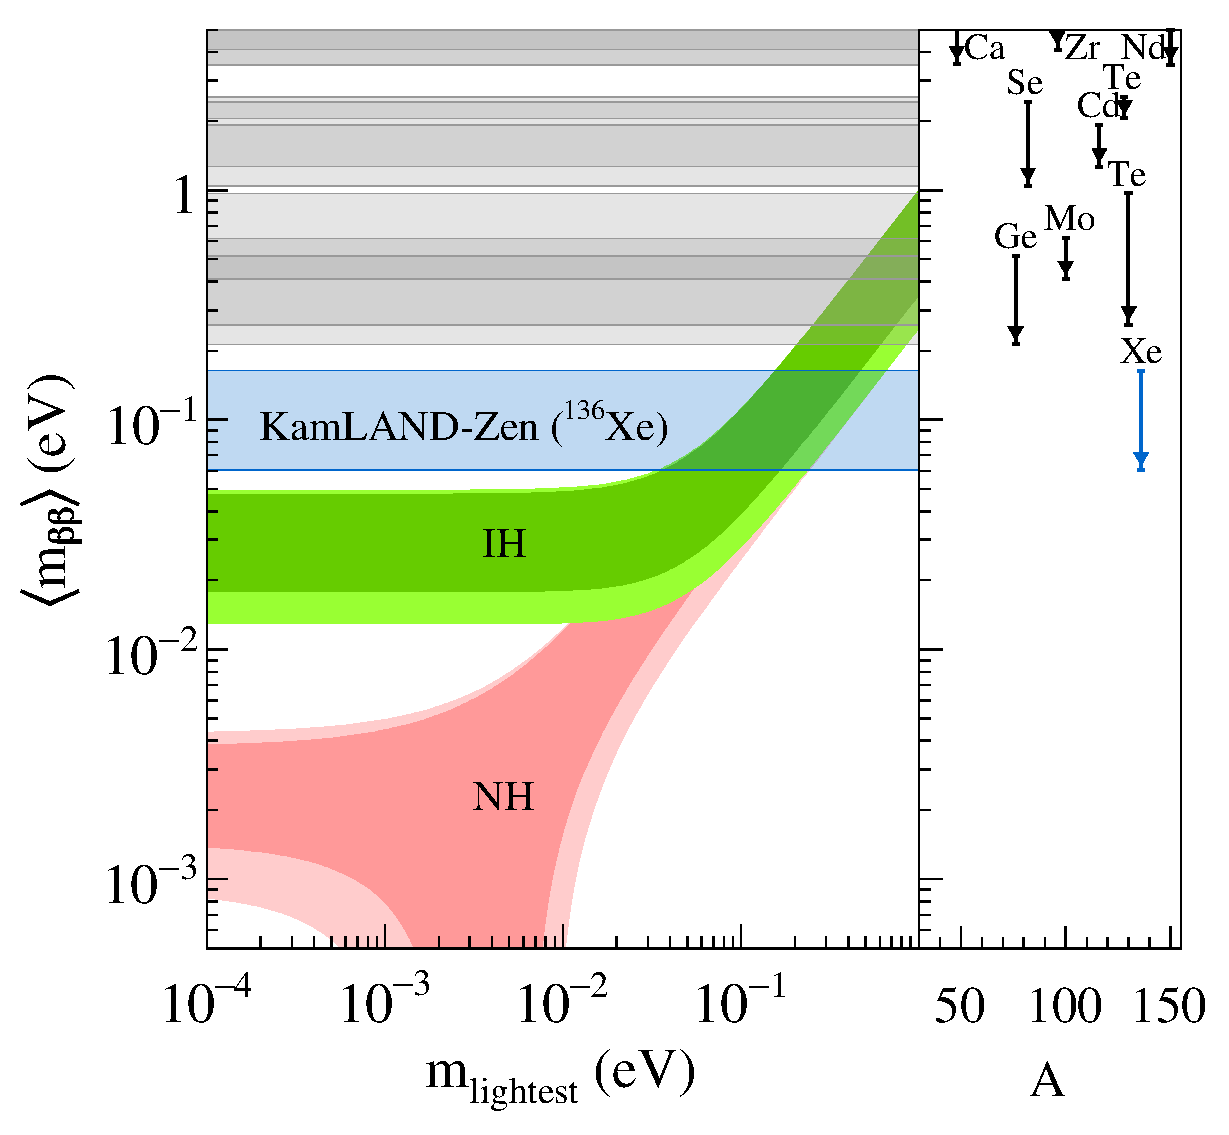
\includegraphics[scale=0.60]{pictures/Chap2/KamLaNDZenResults.pdf}
\caption{Effective neutrino mass (|<m$_{\nu}$>| = m$_{\text{eff}}$) as a function of the lowest mass eigenstate (m$_\text{0}$). The blue band represents the new limits set by KamLAND-Zen with $^{\text{136}}$Xe which is close to the inverted ordering region. The grey bands represent the old limit or the limit obtained on the other isotopes. The  side-panel shows the corresponding limits for each nucleus as a function of the mass number.}
\label{KamLAND-Zen-results}
\end{center}
\end{figure}

\FloatBarrier



\begin{table}
\centering
%\small
\begin{tabular}{|c|c|c|c|c|}
\hline
Transition & Q$_{\beta\beta}$~[keV] & $\eta$ [\%] & G$^{\text{2}\nu}$ [y$^{\text{-1}}$] & G$^{\text{0}\nu}$ [y$^{\text{-1}}$] \\
\hline
$^{\text{46}}$Ca $\rightarrow$ $^{\text{46}}$Ti & 987      $\pm$ 4   & 0.035  & 1.148 10$^{\text{-22}}$ & 1.397 10$^{\text{-27}}$\\
\hline
$^{\text{48}}$Ca $\rightarrow$ $^{\text{48}}$Ti$^{\dagger}$ & 4267.98     $\pm$ 0.34   & 0.187  & 3.968 10$^{\text{-17}}$ & 2.439 10$^{\text{-25}}$\\ 
\hline
$^{\text{70}}$Zn $\rightarrow$ $^{\text{70}}$Ge & 1001     $\pm$ 3   & 0.62   & 3.155 10$^{\text{-22}}$ & 2.342 10$^{\text{-27}}$\\ 
\hline
$^{\text{76}}$Ge $\rightarrow$ $^{\text{76}}$Se & 2039.6   $\pm$ 0.9 & 7.61   & 1.305 10$^{\text{-19}}$ & 2.445 10$^{\text{-26}}$\\ 
\hline
$^{\text{80}}$Se $\rightarrow$ $^{\text{80}}$Kr & 130      $\pm$ 9   & 49.8   & 1.220 10$^{\text{-28}}$ & 4.274 10$^{\text{-29}}$\\ 
\hline
$^{\text{82}}$Se $\rightarrow$ $^{\text{82}}$Kr$^{\dagger}$ & 2997.9   $\pm$ 0.3   & 8.73   & 4.348 10$^{\text{-18}}$ & 1.079 10$^{\text{-25}}$\\ 
\hline
$^{\text{86}}$Kr $\rightarrow$ $^{\text{86}}$Sr & 1256     $\pm$ 5   & 17.3   & 3.333 10$^{\text{-21}}$ & 6.369 10$^{\text{-27}}$\\ 
\hline
$^{\text{94}}$Zr $\rightarrow$ $^{\text{94}}$Mo & 1145.3   $\pm$ 2.5 & 17.4   & 2.304 10$^{\text{-21}}$ & 6.369 10$^{\text{-27}}$\\ 
\hline
$^{\text{96}}$Zr $\rightarrow$ $^{\text{96}}$Mo$^{\dagger}$ & 3350.0     $\pm$ 3.5   & 2.8    & 1.927 10$^{\text{-17}}$ & 2.242 10$^{\text{-25}}$\\ 
\hline
$^{\text{98}}$Mo $\rightarrow$ $^{\text{98}}$Ru & 112      $\pm$ 7   & 24.1   & 9.709 10$^{\text{-29}}$ & 6.711 10$^{\text{-29}}$\\ 
\hline
$^{\text{100}}$Mo $\rightarrow$ $^{\text{100}}$Ru$^{\dagger}$ & 3034.40   $\pm$ 0.17   & 9.63   & 9.434 10$^{\text{-18}}$ & 1.754 10$^{\text{-25}}$\\ 
\hline
$^{\text{104}}$Ru $\rightarrow$ $^{\text{104}}$Pd & 1299   $\pm$ 4   & 18.7   & 9.174 10$^{\text{-21}}$ & 1.202 10$^{\text{-26}}$\\ 
\hline
$^{\text{110}}$Pd $\rightarrow$ $^{\text{110}}$Cd & 2013   $\pm$ 19  & 11.8   & 3.984 10$^{\text{-19}}$ & 5.376 10$^{\text{-26}}$\\ 
\hline
$^{\text{114}}$Cd $\rightarrow$ $^{\text{114}}$Sn & 534    $\pm$ 4   & 28.7   & 1.443 10$^{\text{-23}}$ & 1.639 10$^{\text{-27}}$\\ 
\hline
$^{\text{116}}$Cd $\rightarrow$ $^{\text{116}}$Sn$^{\dagger}$ & 2813.50 $\pm$ 0.13   & 7.49   & 8.000 10$^{\text{-18}}$ & 1.894 10$^{\text{-25}}$\\ 
\hline
$^{\text{122}}$Sn $\rightarrow$ $^{\text{122}}$Te & 364    $\pm$ 4   & 4.56   & 1.047 10$^{\text{-24}}$ & 8.621 10$^{\text{-28}}$\\ 
\hline
$^{\text{124}}$Sn $\rightarrow$ $^{\text{124}}$Te & 2288   $\pm$ 1.6 & 5.64   & 1.686 10$^{\text{-18}}$ & 1.055 10$^{\text{-25}}$\\ 
\hline
$^{\text{128}}$Te $\rightarrow$ $^{\text{128}}$Xe & 868    $\pm$ 4   & 31.7   & 8.475 10$^{\text{-22}}$ & 6.993 10$^{\text{-27}}$\\ 
\hline
$^{\text{130}}$Te $\rightarrow$ $^{\text{130}}$Xe$^{\dagger}$ & 2528.9 $\pm$ 2.1 & 2.1   & 4.808 10$^{\text{-18}}$ & 1.698 10$^{\text{-25}}$\\ 
\hline
$^{\text{134}}$Xe $\rightarrow$ $^{\text{134}}$Ba & 847    $\pm$ 10  & 10.4   & 8.621 10$^{\text{-22}}$ & 7.692 10$^{\text{-27}}$\\ 
\hline
$^{\text{136}}$Xe $\rightarrow$ $^{\text{136}}$Ba & 2479   $\pm$ 8   & 8.9    & 4.831 10$^{\text{-18}}$ & 1.812 10$^{\text{-25}}$\\ 
\hline
$^{\text{142}}$Ce $\rightarrow$ $^{\text{142}}$Nd & 1417.6 $\pm$ 2.5 & 11.1   & 7.246 10$^{\text{-20}}$ & 1.812 10$^{\text{-26}}$\\
\hline 
$^{\text{146}}$Nd $\rightarrow$ $^{\text{146}}$Sm & 56     $\pm$ 5   & 17.2   & 4.854 10$^{\text{-30}}$ & 1.418 10$^{\text{-28}}$\\
\hline 
$^{\text{148}}$Nd $\rightarrow$ $^{\text{148}}$Sm & 1928.3 $\pm$ 1.9 & 5.7    & 1.070 10$^{\text{-18}}$ & 1.276 10$^{\text{-25}}$\\
\hline 
$^{\text{150}}$Nd $\rightarrow$ $^{\text{150}}$Sm$^{\dagger}$ & 3371.38 $\pm$ 0.2 & 5.6    & 1.189 10$^{\text{-16}}$ & 8.000 10$^{\text{-25}}$\\ 
\hline
$^{\text{154}}$Sm $\rightarrow$ $^{\text{154}}$Gd & 1251.9 $\pm$ 1.5 & 22.6   & 4.098 10$^{\text{-20}}$ & 4.202 10$^{\text{-26}}$\\ 
\hline
$^{\text{160}}$Gd $\rightarrow$ $^{\text{160}}$Dy & 1729.5 $\pm$ 1.4 & 21.8   & 6.623 10$^{\text{-19}}$ & 1.252 10$^{\text{-25}}$\\ 
\hline
$^{\text{170}}$Gr $\rightarrow$ $^{\text{170}}$Yd & 653.9  $\pm$ 1.6 & 14.9   & 5.495 10$^{\text{-22}}$ & 1.445 10$^{\text{-26}}$\\ 
\hline
$^{\text{176}}$Yb $\rightarrow$ $^{\text{176}}$Hf & 1078.8 $\pm$ 2.7 & 12.6   & 3.067 10$^{\text{-20}}$ & 5.714 10$^{\text{-26}}$\\ 
\hline
$^{\text{186}}$W $\rightarrow$ $^{\text{186}}$Os & 490.3   $\pm$ 2.2 & 28.6   & 1.302 10$^{\text{-22}}$ & 1.439 10$^{\text{-26}}$\\ 
\hline
$^{\text{192}}$Os $\rightarrow$ $^{\text{192}}$Pj & 417    $\pm$ 4   & 41.0   & 5.051 10$^{\text{-23}}$ & 1.299 10$^{\text{-26}}$\\ 
\hline 
$^{\text{198}}$Pt $\rightarrow$ $^{\text{198}}$Hg & 1048   $\pm$ 4   & 7.2    & 6.135 10$^{\text{-20}}$ & 1.144 10$^{\text{-25}}$\\
\hline 
$^{\text{204}}$Hg $\rightarrow$ $^{\text{204}}$Pb & 416.5  $\pm$ 1.9 & 6.9    & 8.130 10$^{\text{-23}}$ & 1.976 10$^{\text{-26}}$\\
\hline 
$^{\text{232}}$Th $\rightarrow$ $^{\text{232}}$U & 858     $\pm$ 6   & 100    & 5.952 10$^{\text{-20}}$ & 2.519 10$^{\text{-25}}$\\
\hline 
$^{\text{238}}$U $\rightarrow$ $^{\text{238}}$Pu & 1145.8  $\pm$ 1.7 & 99.275 & 6.803 10$^{\text{-19}}$ & 5.952 10$^{\text{-25}}$\\ 
\hline
\end{tabular}
\caption{Transition energy, natural abundance and space phase factors of the 35 $\beta^{-}$ isotopes from~\cite{ParameterBBisotopes} except the values marked by a $^{\dagger}$ where Q$_{\beta\beta}$ uncertainties have been updated.}
\label{tab:2nuIsotopes}
\end{table}


\FloatBarrier


\end{document}
